\documentclass[12pt,a4paper]{article}
\usepackage[utf8]{inputenc}
\usepackage[english]{babel}
\usepackage{amsmath}
\usepackage{adjustbox}
\usepackage{amsfonts}
\usepackage{csquotes}
\usepackage{float}
\usepackage{amssymb}
\usepackage{minted}
\usepackage{pdflscape}
\usepackage[toc,page]{appendix}
\usepackage{fancyvrb}
\usepackage{multirow}
\usepackage{graphicx}
\DeclareMathOperator*{\argmax}{arg\,max}
\DeclareMathOperator*{\argmin}{arg\,min}
\usepackage{setspace}
\usepackage{breakcites}
\usepackage{tikz}
\usetikzlibrary{arrows.meta}
\renewcommand{\floatpagefraction}{.8}%
\usepackage{varioref}
\usepackage{caption}
\usepackage{subcaption}
\usepackage{lscape}
\usepackage[acronym, indexonlyfirst]{glossaries}
\usepackage{booktabs}
\usepackage{capt-of}
\usepackage{wrapfig}
\usepackage{booktabs}
\usepackage[nottoc]{tocbibind}
\usepackage{array}
\usepackage{multirow}

\newcommand\MyBox[2]{
  \fbox{\lower0.75cm
    \vbox to 1.7cm{\vfil
      \hbox to 1.7cm{\hfil\parbox{1.4cm}{#1\\#2}\hfil}
      \vfil}%
  }%
}
\makeglossaries
%\input{acros}
\newcommand{\ts}{\textsuperscript}
\usepackage[toc,page]{appendix}
\onehalfspacing
\usepackage[left=2cm,right=2cm,top=2cm,bottom=2cm]{geometry} %check before printing: Increase left margin
\newcommand{\HRule}{\rule{\linewidth}{0.5mm}}
\author{Marius Breitling}
\title{Master Thesis}
\begin{document}
%description: Deckblatt in Deutsch
%% Basierend auf einer TeXnicCenter-Vorlage von Tino Weinkauf.
%%%%%%%%%%%%%%%%%%%%%%%%%%%%%%%%%%%%%%%%%%%%%%%%%%%%%%%%%%%%%%

%%%%%%%%%%%%%%%%%%%%%%%%%%%%%%%%%%%%%%%%%%%%%%%%%%%%%%%%%%%%%
%% Deckblatt
%%%%%%%%%%%%%%%%%%%%%%%%%%%%%%%%%%%%%%%%%%%%%%%%%%%%%%%%%%%%%
%%
%% ACHTUNG: Sie benötigen ein Hauptdokument, um diese Datei
%%          benutzen zu können. Verwenden Sie im Hauptdokument
%%          den Befehl "\input{dateiname}", um diese
%%          Datei einzubinden.
\begin{titlepage}

\begin{center}


% Upper part of the page
%\includegraphics[width=0.15\textwidth]{./logo}\\[1cm]    

\textsc{\LARGE University of Konstanz}\\[1.5cm]
%\includegraphics[scale=0.1]{UniKonstanz_Logo_Optimum_SW.eps}
% Title
\HRule \\[0.4cm]
{\LARGE \bfseries \begin{center}Banking Default Prediction and the Class Imbalance Problem\\
 - Data Analysis Project - 
%A Machinelearning Approach
}\\[0.4cm]
\HRule \\[1.5cm]


% Author and supervisor
\end{center}
\begin{center}
%\bfseries
\normalsize
\end{center}
\vfill
\begin{flushleft}
\bfseries
\normalsize
Submitted by:\\
Marius Breitling\\
Struempfelbacherstr. 258\\
71384 Weinstadt\\
\vspace{15pt}
Summer Term 2019\\
\vspace{15pt}
Supervisor: Assistant Professor Lyudmila Grigoryeva\\
\vspace{15pt}
Dortmund, \today
\end{flushleft}
\end{titlepage}
\clearpage
\pagenumbering{Roman}
\setcounter{page}{2}
\newgeometry{left=4cm,right=2cm,top=2cm,bottom=2cm}
\tableofcontents
\printglossary[type=\acronymtype]
\pagebreak
\newgeometry{left=4cm,right=2cm,top=2cm,bottom=2cm}
\pagenumbering{arabic}
\section{Introduction}
The defaults of banks and other financial institutes can have shattering consequences for whole economies and are of therefore of highest concern. At the latest since the subprime mortgage market crisis in the US and the following full grown financial crisis starting in 2008 the question how banking defaults can be predicted reliably is of higher interest than ever. Could appropriate countermeasures have softened the severe consequences of banking defaults, as the one of Lehman Brothers in the third quarter of 2008, if it would have been predicted early enough? This small project is evaluating the application of a machine learning algorithm based on several indicators following the CAMELS (\enquote{Capital adequacy, Asset quality, Management, Earnings, Liquidity, and Sensitivity}) rating system to predict the failure of banks. The key point is the question how problems associated with a severe imbalance in the distribution of the target variable can be overcome. Machine learning algorithms often do have problems during their implicit optimization procedures if the outcome variable is highly skewed towards one of its outcomes. We therefore examine alternatives to common measures of accuracy used in the machine learning context and assess to which level we can improve the outcome by synthetically oversampling the minority class of the target variable. For this purpose we're using the approach of SMOTE (\enquote{Synthetic Minority Oversampling Technique}) to provide the algorithm with a more balanced training set.\par
Besides the problems of imbalance, we are looking at a usual binary classification problem in a supervised context. So one of the main problems besides an imbalanced target variable will just be the parameter tuning of the applied model. For our purpose we're trying to assess how a Gradient Boosting Machine (GBM) is performing and which effect the oversampling of the minority class might have on the model's performance.
\section{The Learning of Rare Instances}
\subsection{Performance Measures in the Machine Learning Context}
Aggwarwal \cite{aggarwalClassBook} describes the learning or classification of rare instances basically as the supervised counterpart to outlier detection in an unsupervided framework. He points out that because of the very nature of such a problem, the \enquote{rare nature of anomalies} and the following limited availability of data, it is often \enquote{hard to create robust and generalized models} on the basis of such data. \par
As we will see later, this paper is limited to a binary classification problem why the resulting confusion matrix will have the form of the 2 x 2 matrix in Table \vref{confusion_matrix} \cite{aggarwalClassBook}.\par
\begin{table}
\begin{center}
\begin{tabular}{c|c|c|c|c}
\multicolumn{2}{c}{}&\multicolumn{2}{c}{Predicted Class}&\\
\cline{3-4}
\multicolumn{2}{c|}{}&Pred. Positive&Pred. Negative&\multicolumn{1}{c}{$\Sigma$}\\
\cline{2-4}
\multirow{2}{*}{Real Class}& Actual Positive & $a$ (TP) & $b$ (FN) & $a+b$\\
\cline{2-4}
& Actual Negative & $c$ (FP) & $d$ (TN) & $c+d$\\
\cline{2-4}
\multicolumn{1}{c}{} & \multicolumn{1}{c}{$\Sigma$} & \multicolumn{1}{c}{$a+c$} & \multicolumn{    1}{c}{$b+d$} & \multicolumn{1}{c}{$N$}\\
\end{tabular}
\end{center}
\caption{Confusion matrix for a binary classification problem}
\label{confusion_matrix}
\end{table}
Looking at the matrix, we can easily carve out why common performance measures and an optimization procedure according to them can be problematic in the case of a heavily skewed distribution of the target variable \cite{chawla2002smote}. The most straightforward, and also quite common, performance measure in a classification framework is the accuracy rate, defined as the ratio of correctly classified observations and the total number of observations. We can write the accuracy of an arbitrary classifier $c$ as
\begin{align*}
    acc(c) &= \frac{TP + TN}{TP + TN + FP + FN}\\
    &= \frac{a +  d}{a + b + c + d}\\
    &=1-err(c).
\end{align*}
Often the rare observations within the population are those of the highest interest. Common examples are the detection of a comparably small number of fraudelent among a lot of legitimate credit card transactions or the automatic detection of mammography images or radiographs showing cancerous cells by contrast to healthy material. The very intention of a classification algorithm is the recognition of the minority observations in those and a lot of other cases. Given that early cancer detection can be life saving, it is self evident how costly the misclassification of those problematic cases actually can be. In those areas it might be even tolerable to sacrifice some of the right predictions in the majority class in favor of more predictive power in the minority class - a trade off which we'll have a look at later on. \par
The problem at hand stems from a whole other area but has one thing in common: A learning algorithm is actually applied to identify those rare cases why the maximization of the vanilla accuracy rate doesn't tell you anything useful about the classification quality. An algorithm applied to a population with a 99.9\% to 0.01\% ratio of the majority and the minority class, would achieve an accuracy rate near to 100\% when naively assigning each single observation to the majority class while completely failing its actual purpose of identifying banks which might be likely to fail and cause a lot of economical damage. In the area of learning from imbalanced datasets there are common alternative performance measures to the simple accuracy as shown by Fernandez et al. \cite{fernandez2018learning}:\par
One straightforward alternative is the usage of \textit{precision}, \textit{recall (also called sensitivity)} and a combined measure in the form of the weighted harmonic mean of both (\textit{F-measure}), or their geometric mean (\textit{G-measure}). Be aware that the words \enquote{recall} and \enquote{sensitivity} are used as synonyms in this paper. Although this list is far from exhaustive considering the wide range of existing alternatives, we will stick to those most common measure and come back to those later in the analysis. The measures are defined as follows \cite{fernandez2018learning}:
\begin{align*}
recall&=\frac{TP}{TP + FN}=\frac{a}{a+b}\\
precision&=\frac{TP}{TP + FP}=\frac{a}{a+c}\\
specifity&=\frac{TN}{TN+FP}=\frac{d}{c+d}\\
    F_\beta &= (1+\beta^2)\frac{precision\cdot recall}{(\beta^2 \cdot precision)+recall}\\
    \intertext{where in the standard form $\beta$ is usually set to 1:}\\
    F_1&=2\frac{precision\cdot recall}{precision + recall}\\
    G-measure&=\sqrt{precision\cdot recall}
\end{align*}
There obviously is a tradeoff between the recall and the precision of a classifier. Which of both you actually want to maximize has to be based on the goals of the classification problem and how conservative your estimation actually should be. Maximizing the recall means that the algorithm is able to correctly classify most of the relevant (positive) cases (high TP and low FN). A high recall is particularly important if the misclassification of a relevant case (as FN) might be very costly. An HIV test is a good example for this. You are willing to rather sacrifice some precision (higher FPR) in favor of a better recall to make sure that every HIV positive person is correctly tested. The same could be said for our scenario, we are more interested in getting a broader prediction of potentially failing banks, which we examine in more detail by having a closer look at their books while it might be not as problematic to misclassify some banks which will actually operate successfully.

As another approach to measure model performance, which is particularly useful when dealing with imbalanced datasets, Fernandez et al. point out the more graphical approach of the ROC-curve (Receiver Operating Characteristics) and the closely related AUC (Area Under the Curve). The ROC-curve plots the True-Positive-Rate (TPR) of a classifier for each given False-Positive-Rate (FPR). 

For a broad overview over machine learning applications dealing with imbalanced data sets see \cite{fernandez2018learning}. Fernandez et al. also make clear that usually it's not the imbalanced target distribution itself which prevents an algorithm from learning, but rather the problems which come along with the imbalance. They point out that the main problem is not necessarily the imbalance but rather the lack of training examples from the minority class, which is a consequence of the imbalance. The error rate would decrease if it would be possible to gather enough overall observations to guarantee that there are a sufficient number of observations in both groups. Another mentioned problem is the overlapping feature space of the minority and majority class. If we assume that there was no overlap at all between the two spaces, an algorithm would be able to classify the observations in a satisfying manner even if the distribution is highly skewed towards one of the classes.

Two points described by Aggarwal, which will lead us to SMOTE, are the paucity of training data and the danger of overfitting the minority class \cite{aggarwalClassBook}. This obviously holds even for more or less large datasets: While you're delivered with abundant data belonging to the majority class, there might be not enough data for training an algorithm which generalizes well on a test set, but only manages to capture the characteristics inherent to the available training data.\par
Aggarwal classifies the techniques to overcome the problems going along with a severe class imbalance into two categories:
\begin{itemize}
    \item Cost Sensitive Learning
    \item Adaptive Re-sampling
\end{itemize}
While the first technique modifies the cost function which is subject to the algorithm's optimization problem, for example by overweighting the costs for a misclassification in the minority group, the second rather tries to grab the problem at the root by applying different sampling techniques to the training data. By this measure one wants to reach a more balanced training data set. In this paper I'm going to focus on the technique SMOTE, which is an example of a re-sampling technique:
\subsection{SMOTE}
Fernandez et al. name three categories of resampling approaches to the imbalance problem \cite{fernandez2018learning}:
\begin{enumerate}
    \item Undersampling methods
    \item Oversampling Methods
    \item Hybrid Methods
\end{enumerate}
As the name of SMOTE suggests it is part of the second group (\enquote{Synthetic Minority Oversampling Technique}). Pseudo-code for the algorithm can be found in the original paper \cite{chawla2002smote} or in \cite{fernandez2018learning}. We're leaving the reader with a rough sketch of the algorithm instead. While there are simpler algorithms which are just trying to randomly resample existing data, SMOTE's goal is to oversample the minority group by creating new synthetic minority observations. New observations are created by means of linear combinations of existing minority data points. The rough sketch is as follows, where $N\cdot100\%$ is said to be the oversampling rate. A rate of $100\%$ results in a duplication of the number of minority observations, a rate of $200\%$ in a triplication and so on.
\begin{enumerate}
    \item For each minority data point $x_i$ compute its $K$ nearest neighbors $x_{ik}$ for $k \in [1,K]$.
    \item Among those neighbors sample randomly $N$ data points.
    \item For each of the points compute a random linear combination of the original point and the respective nearest neighbor.
    \item Each of the linear combinations delivers a new synthetic observation of the form:
    \item $r_k = x_i + t\cdot\left(x_{ik}-x_i\right)$ where $t$ is a random variable from the real interval $[0,1]$
\end{enumerate}
SMOTE can also be extended to nominal features, which is not relevant for the application at hand. For this purpose a majority voting of the chosen nearest neighbors is executed for the nominal feature and the value with highest voting is adapted. Ties are usually just broken at random \cite{chawla2003smoteboost}.
Figure \ref{fig:smote_vis_1} on page \pageref{fig:smote_vis_1} and Figure \ref{fig:smote_vis_2} on page \pageref{fig:smote_vis_2} offer a visualization how SMOTE actually works in practice. For the sake of simplicity I generated two totally random and normally distributed two dimensional datasets and implemented a rough version of SMOTE in R. The Minority class (black) is distributed according to a normal distribution with mean $0.1$ and a standard deviation of $0.4$. For the majority group the respective measures are $0.6$ and $0.3$. In this very simple example, which was just implemented for the pure purpose of visualizing a few steps of SMOTE, we are iterating over each of the original minority points. The point, which is drawn at the specific step is marked in blue. For that point its 5 nearest neighbors are computed ($k=5$, drawn in orange) and four of the neighbors ($n=4$) are sampled randomly. The minority group originally consists of 50 observations by contrast to the majority group which contains 5000 observations which leaves is with a ratio of $\frac{1}{100}$ of the minority to the majority class. 

The synthetic observations are then created on a random point on the linear combination between the original point and its chosen neighbors. The new points, which are drawn in green, are added to the minority group and the algorithm moves to the next step. The figures show the first four and the two last steps of the algorithm, in the left column of each graphic the complete dataset is shown, the right column of each graphic shows a zoomed, more detailed image of the step. Because we're only iterating once over the original data points (and $n=4$) the minority data set is augmented by 200 additional observations which gives us a ration of $\frac{1}{20}$ after Step 50, which is obviously still far from balanced but enough to show what is going on behind the curtains of SMOTE. The nearest neighbors computation was not implemented by myself but done by means of the \verb+nn2+ function of the R \nocite{pack:r_base} package \verb+RANN+, which offers a very fast nearest neighbor search implemented on a kd-tree, which is running in $\mathcal{O}(m\log{m})$ \cite{Arya2019}. The resulting visualizations for all 50 steps, separately and merged (\verb+./Graphics/Smote Visualization/smote_accumulating.gif+) to an interactive GIF can be found in the public GitHub-Repository providing supplementary material to this project \cite{publicRepo}. On top of that the underlying source code (\verb+./Sources/smote_vis_accumulating.r+) and a rough and simple Python implementation (\verb+./Sources/smote.py+) is provided.
\begin{figure}[] % "[t!]" placement specifier just for this example
\begin{subfigure}{0.48\textwidth}
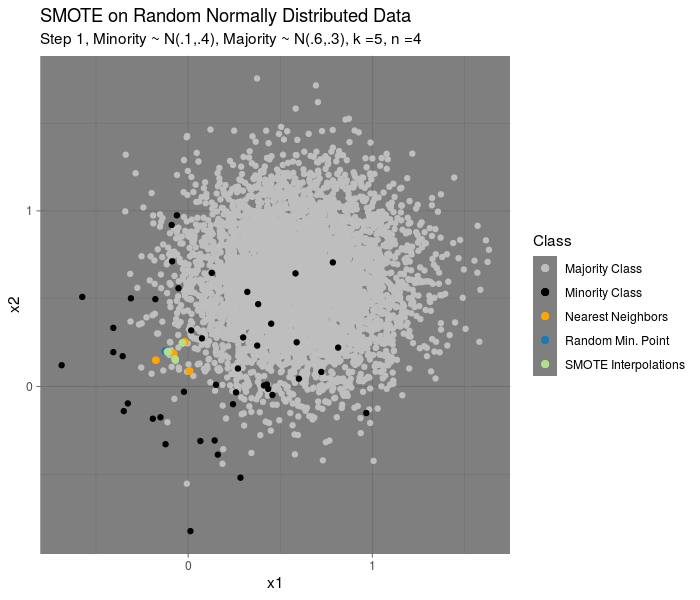
\includegraphics[width=\linewidth]{./graphics/knn001.png}
\caption{SMOTE Visualization: Step 1} \label{fig:a}
\end{subfigure}\hspace*{\fill}
\begin{subfigure}{0.48\textwidth}
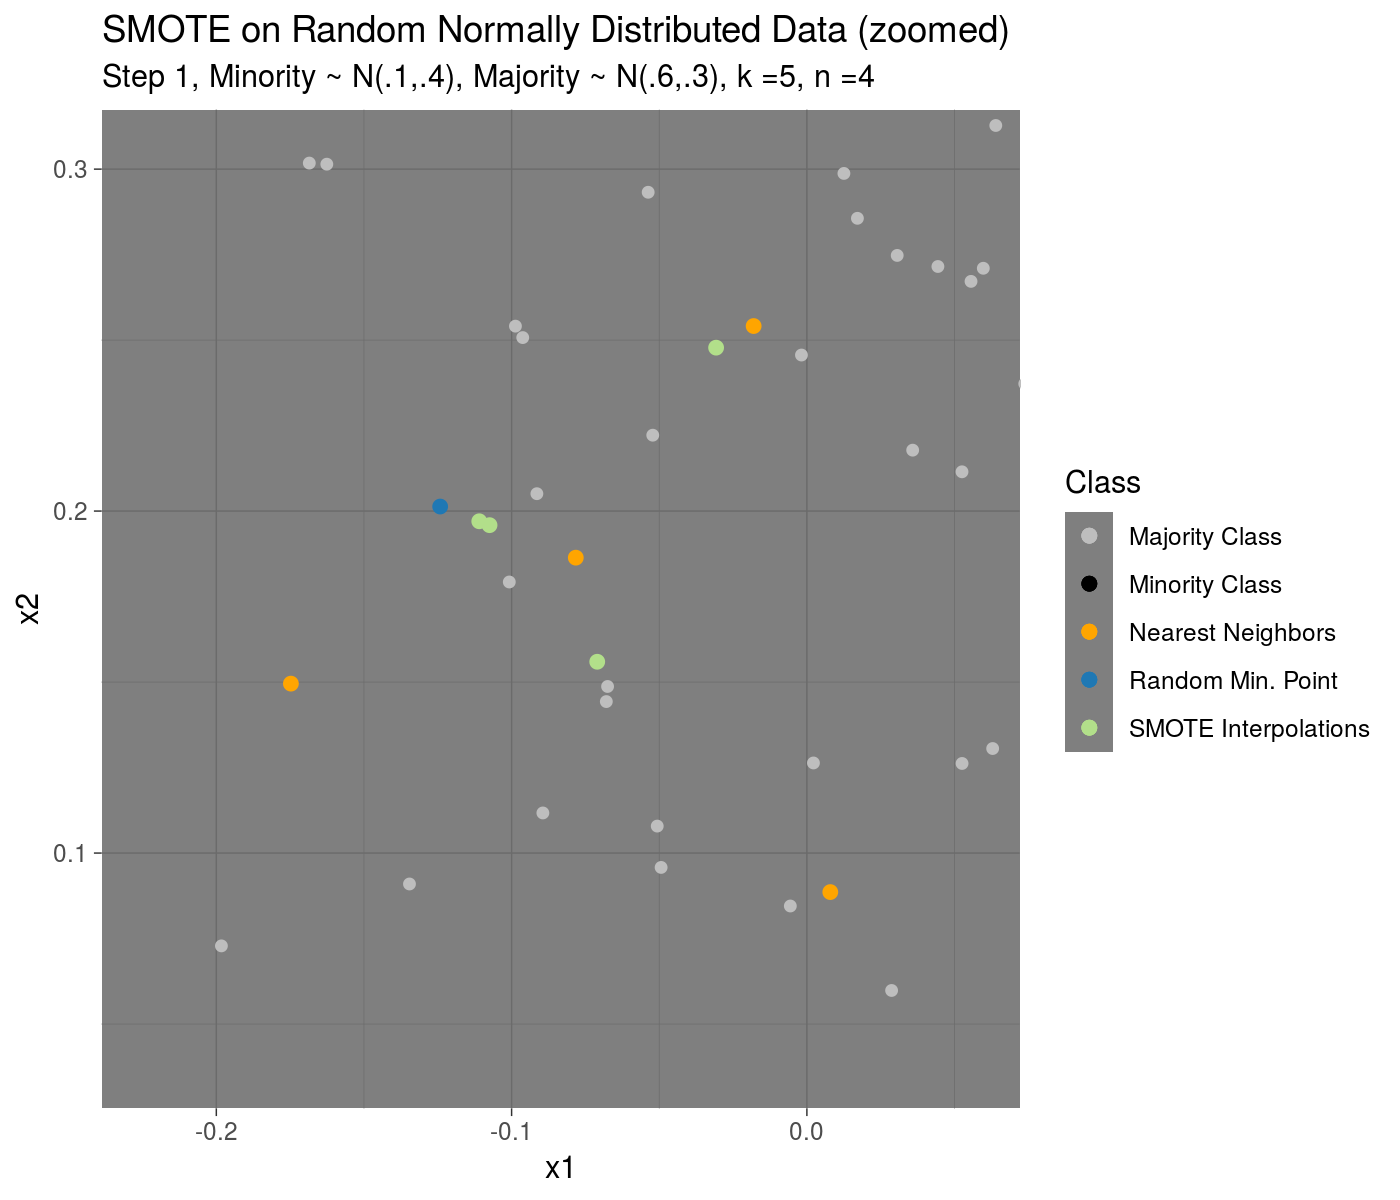
\includegraphics[width=\linewidth]{./graphics/knn_zoom001.png}
\caption{SMOTE Visualization: Step 1 - zoomed} \label{fig:b}
\end{subfigure}
\medskip
\begin{subfigure}{0.48\textwidth}
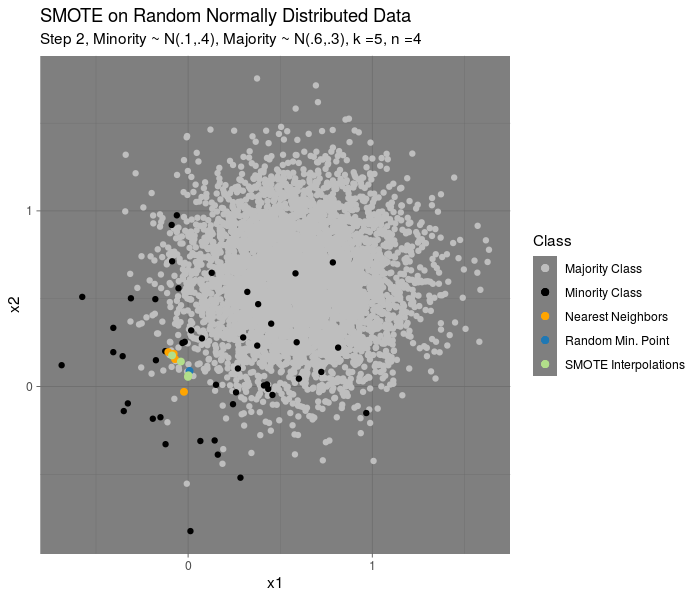
\includegraphics[width=\linewidth]{./graphics/knn002.png}
\caption{SMOTE Visualization: Step 2} \label{fig:a}
\end{subfigure}\hspace*{\fill}
\begin{subfigure}{0.48\textwidth}
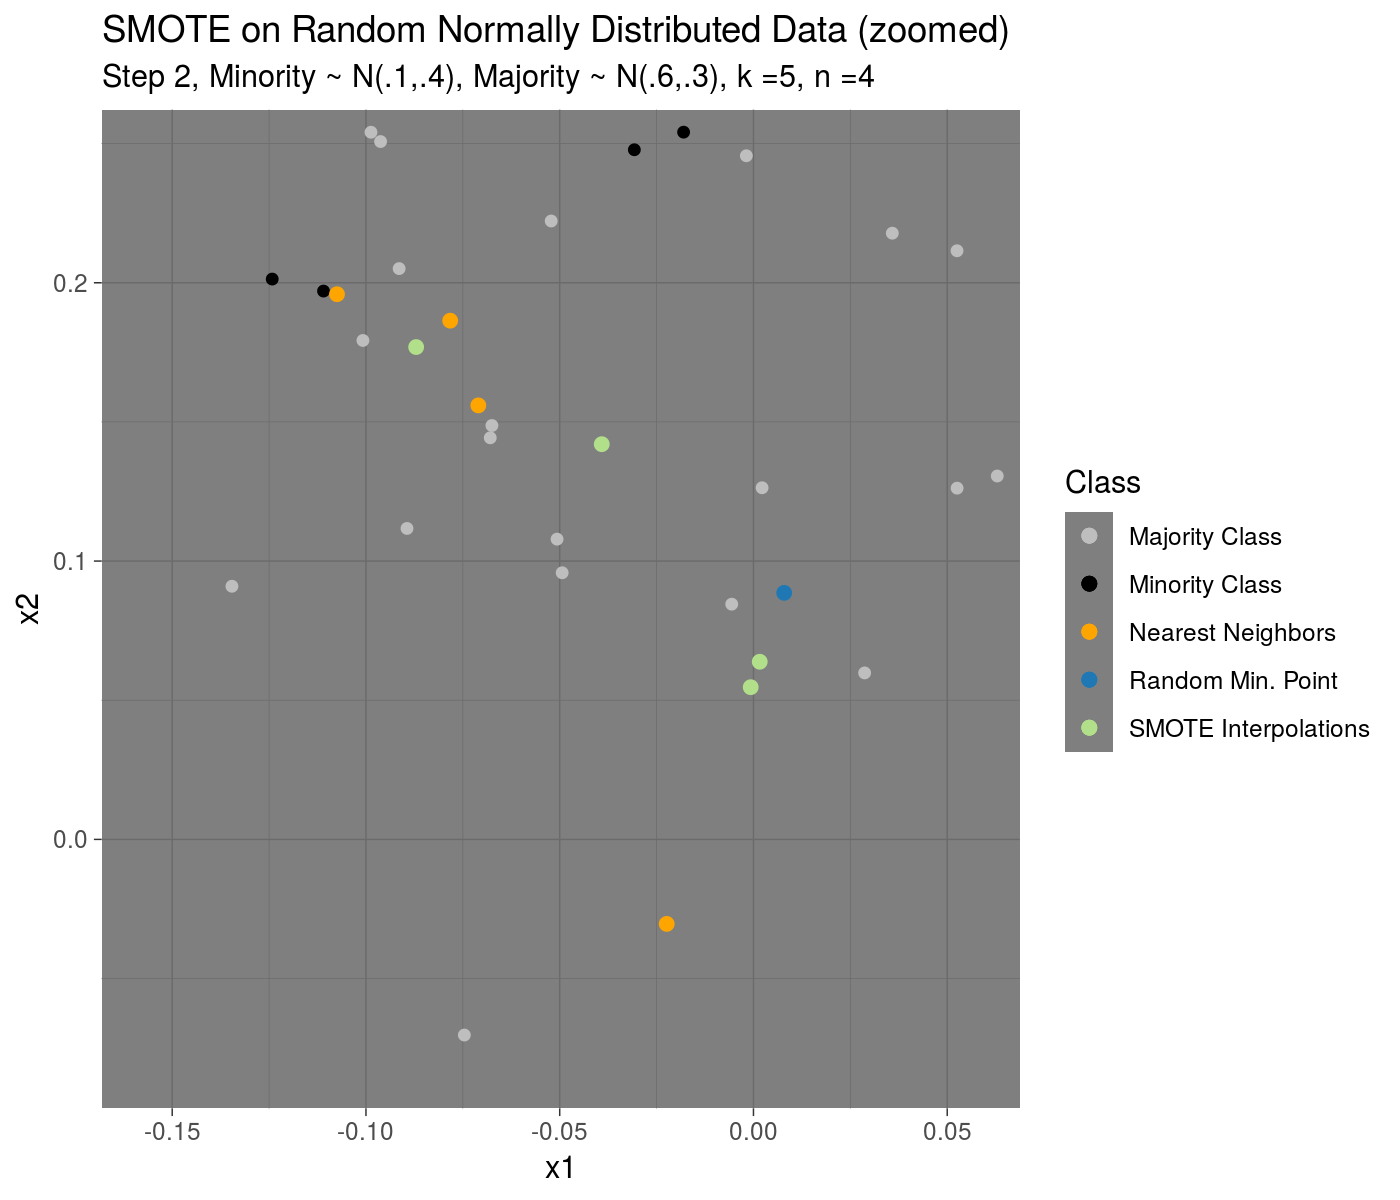
\includegraphics[width=\linewidth]{./graphics/knn_zoom002.png}
\caption{SMOTE Visualization: Step 2 - zoomed} \label{fig:a}
\end{subfigure}
\medskip
\begin{subfigure}{0.48\textwidth}
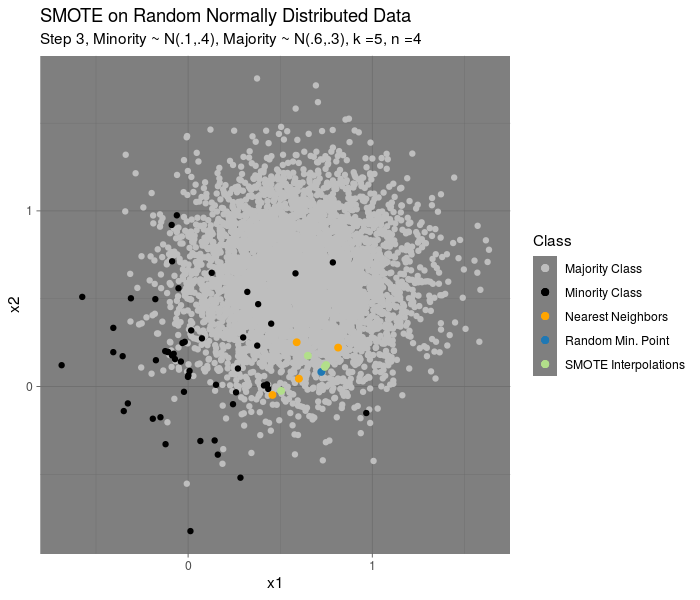
\includegraphics[width=\linewidth]{./graphics/knn003.png}
\caption{SMOTE Visualization: Step 3} \label{fig:a}
\end{subfigure}\hspace*{\fill}
\begin{subfigure}{0.48\textwidth}
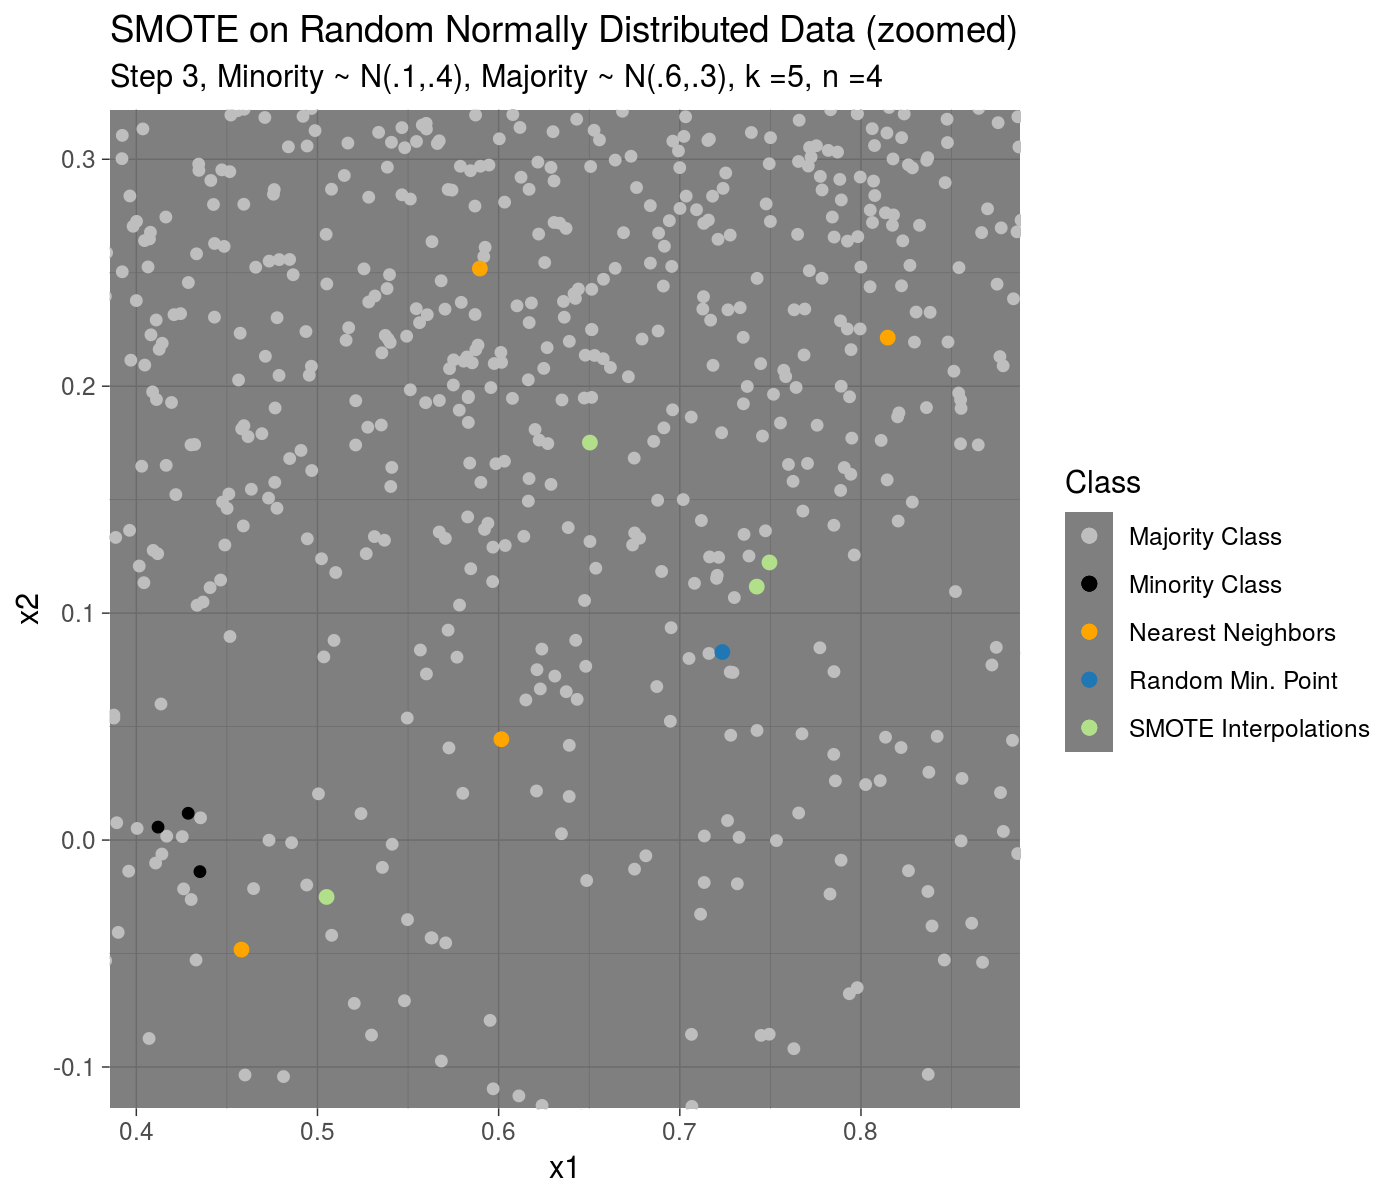
\includegraphics[width=\linewidth]{./graphics/knn_zoom003.png}
\caption{SMOTE Visualization: Step 3 - zoomed} \label{fig:a}
\end{subfigure}
\caption{SMOTE visualization, Steps 1, 2, 3} \label{fig:smote_vis_1}
\end{figure}
\begin{figure}[] % "[t!]" placement specifier just for this example
\begin{subfigure}{0.48\textwidth}
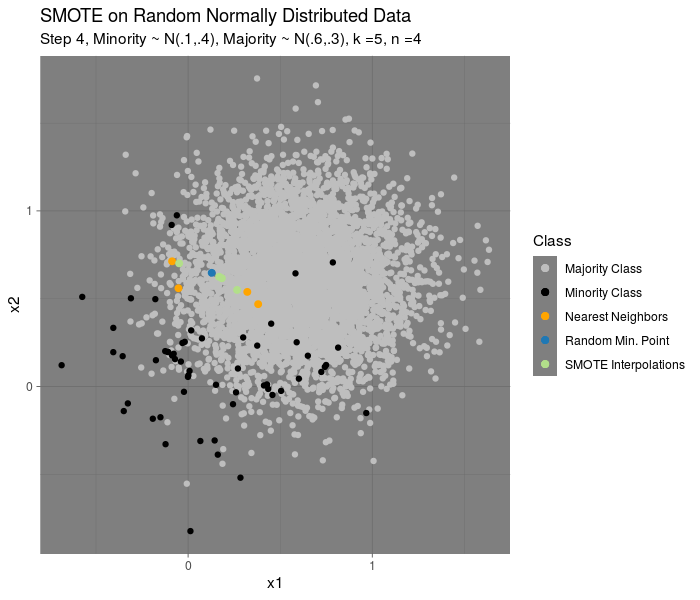
\includegraphics[width=\linewidth]{./graphics/knn004.png}
\caption{SMOTE Visualization: Step 4} \label{fig:a}
\end{subfigure}\hspace*{\fill}
\begin{subfigure}{0.48\textwidth}
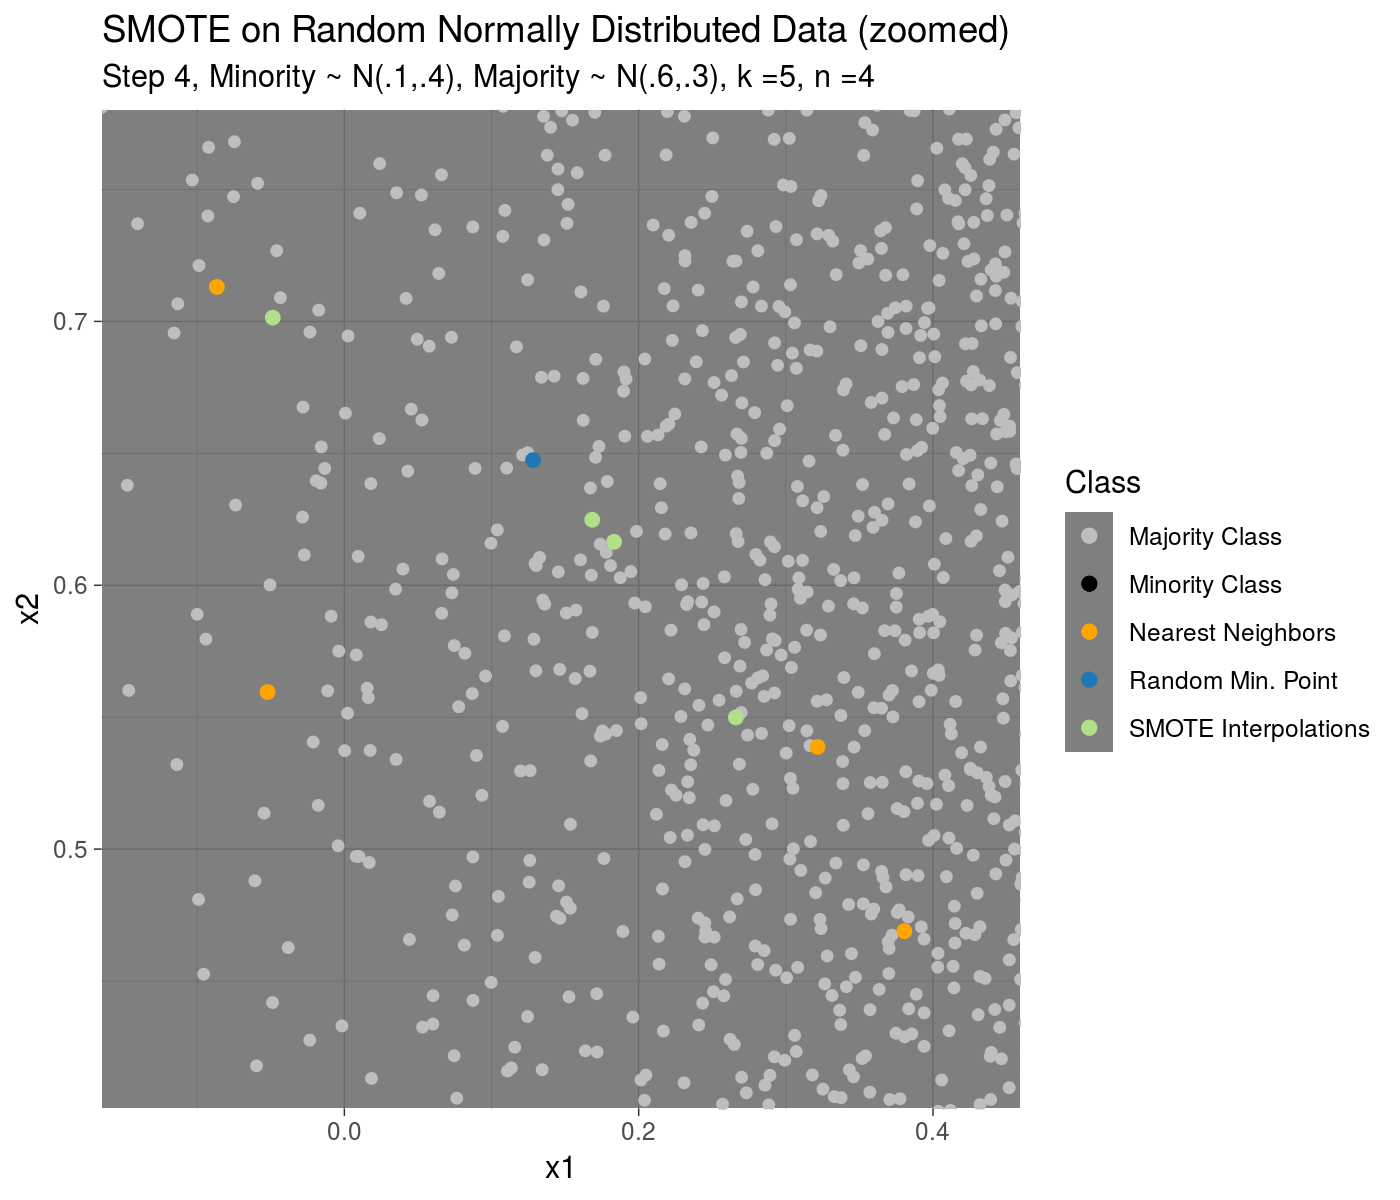
\includegraphics[width=\linewidth]{./graphics/knn_zoom004.png}
\caption{SMOTE Visualization: Step 4 - zoomed} \label{fig:a}
\end{subfigure}
\medskip
\begin{subfigure}{0.48\textwidth}
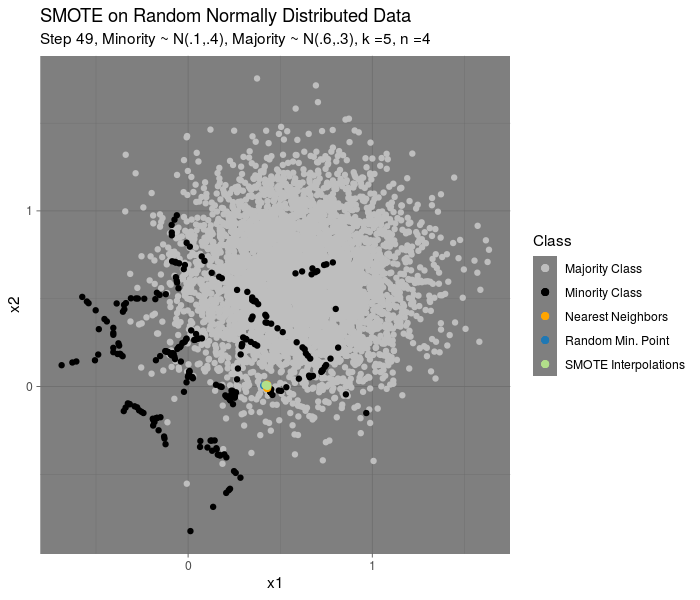
\includegraphics[width=\linewidth]{./graphics/knn049.png}
\caption{SMOTE Visualization: Step 49} \label{fig:a}
\end{subfigure}\hspace*{\fill}
\begin{subfigure}{0.48\textwidth}
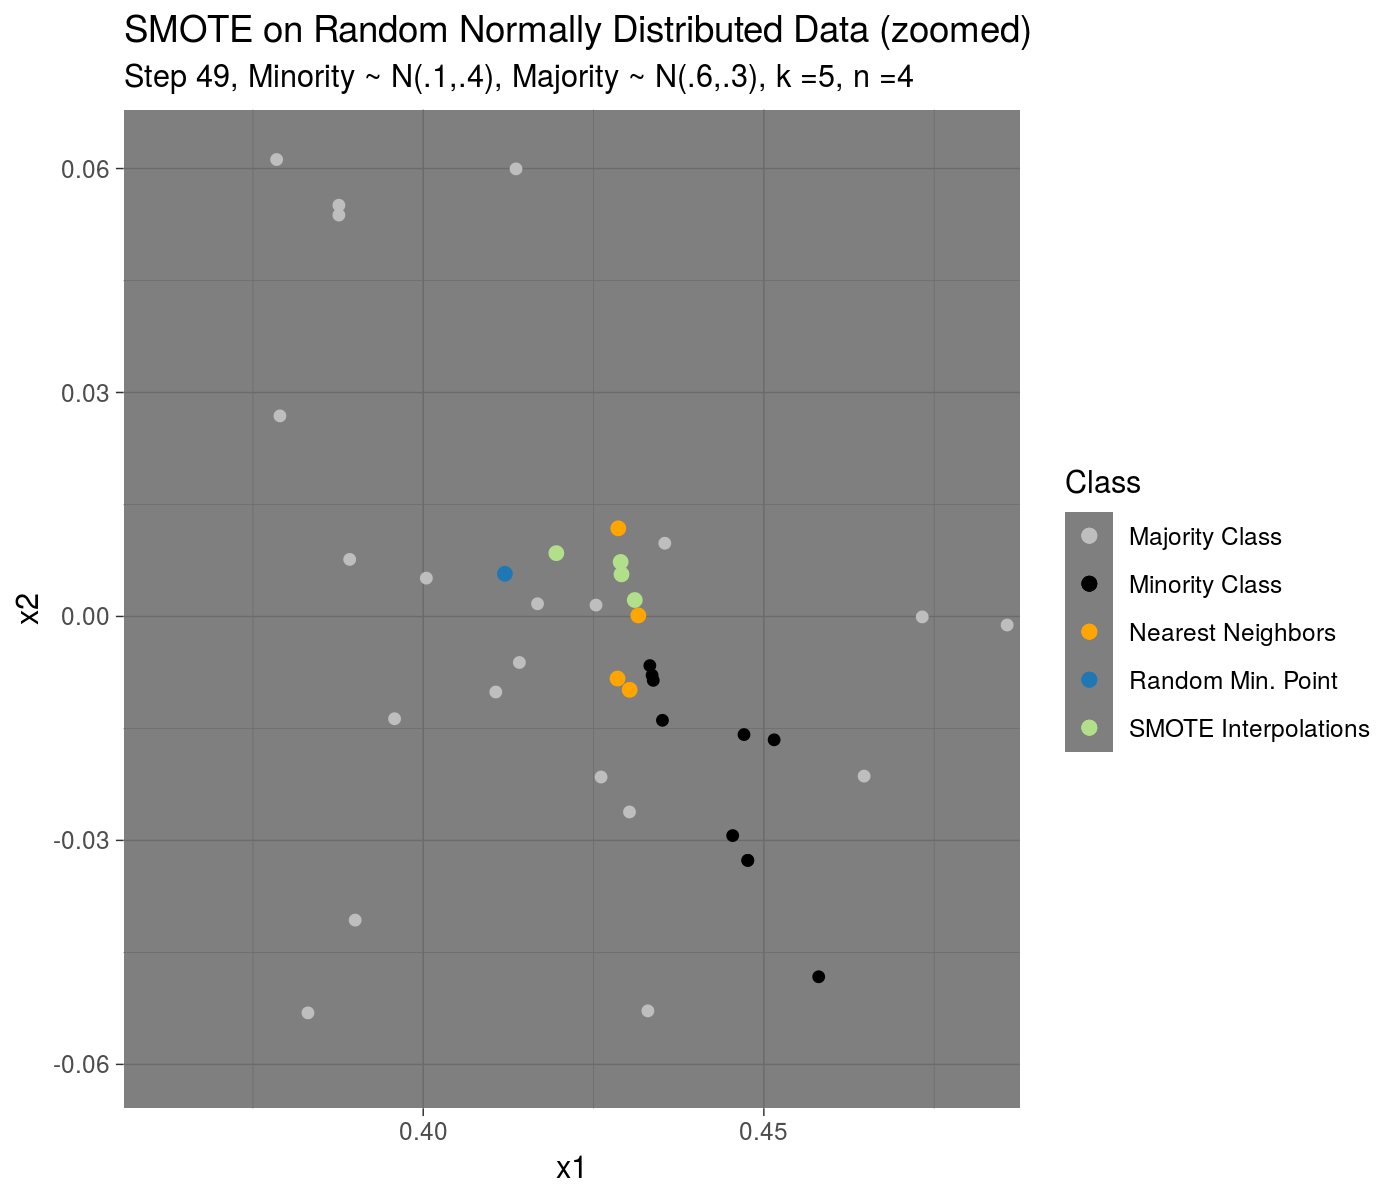
\includegraphics[width=\linewidth]{./graphics/knn_zoom049.png}
\caption{SMOTE Visualization: Step 49 - zoomed} \label{fig:a}
\end{subfigure}
\medskip
\begin{subfigure}{0.48\textwidth}
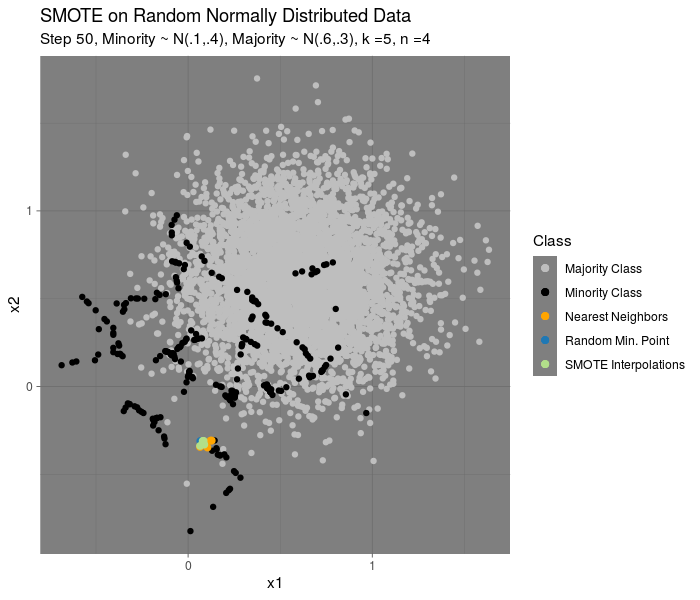
\includegraphics[width=\linewidth]{./graphics/knn050.png}
\caption{SMOTE Visualization: Step 50} \label{fig:a}
\end{subfigure}\hspace*{\fill}
\begin{subfigure}{0.48\textwidth}
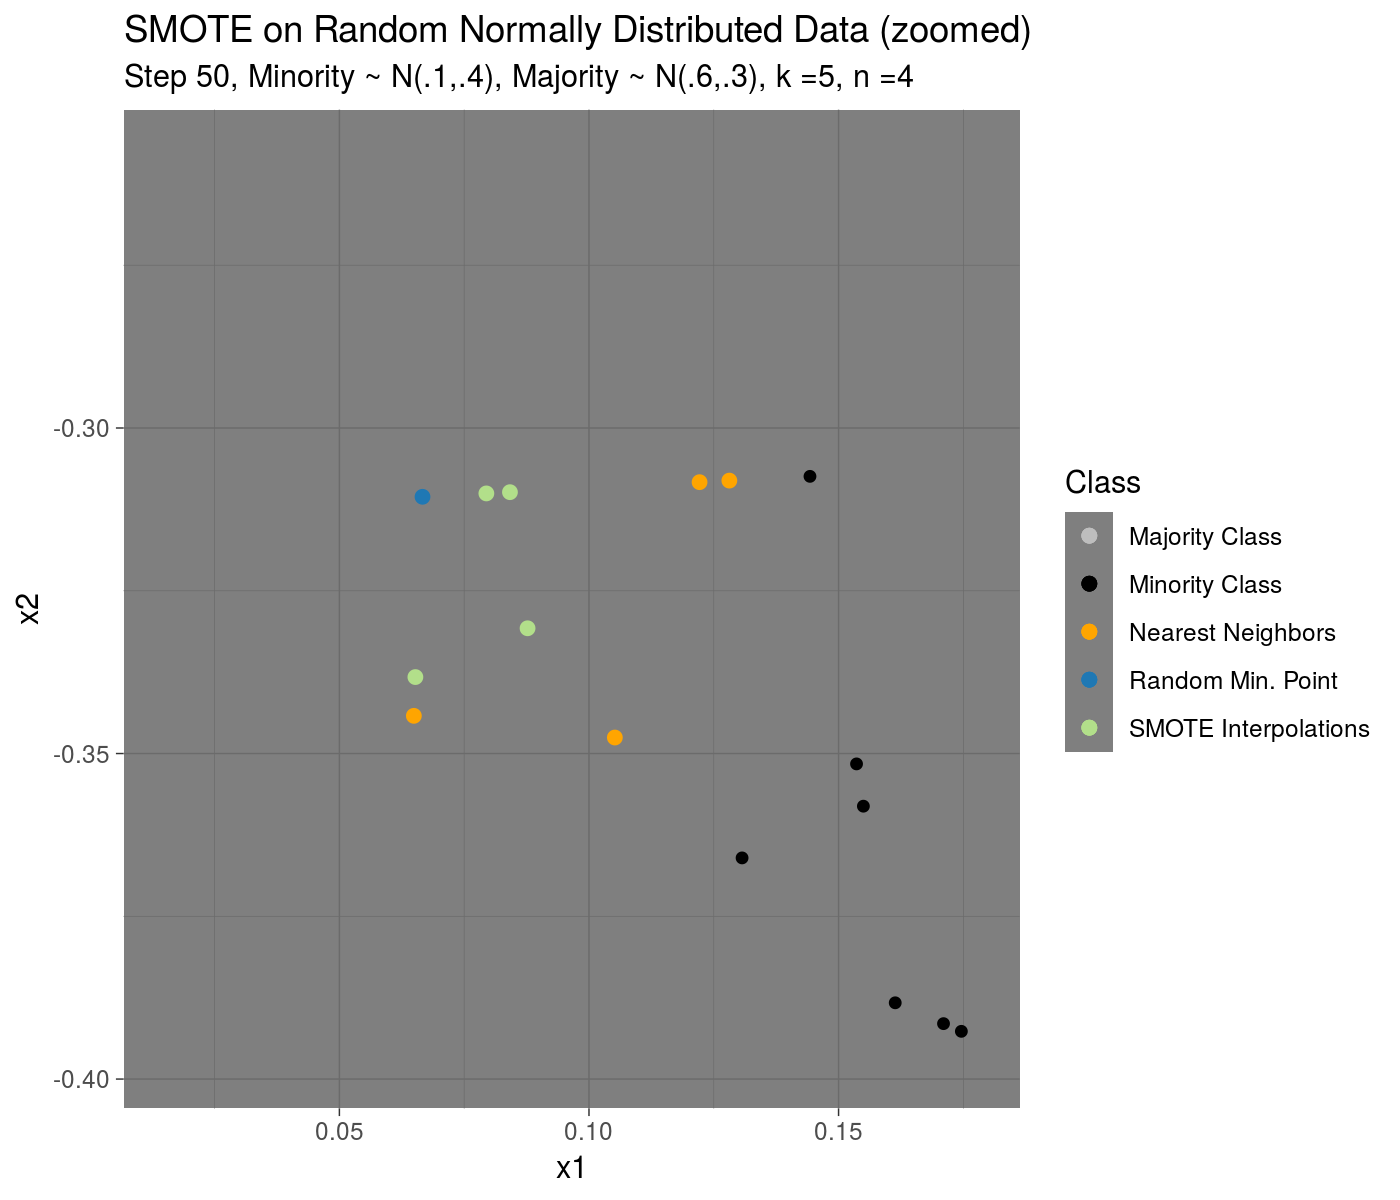
\includegraphics[width=\linewidth]{./graphics/knn_zoom050.png}
\caption{SMOTE Visualization: Step 50 - zoomed} \label{fig:a}
\end{subfigure}
\caption{SMOTE visualization, Steps 4, 49, 50} \label{fig:smote_vis_2}
\end{figure}
\section{Dataset}
\subsection{Description}
This project is based on the dataset delivered as \verb+Dataset_large.RData+, which contains 357,696 observations measured in 58 variables. Each single row contains one single bank at a certain quarter in time. This specific dataset contains measurements of 9936 banks measured at 36 subsequent periods, more precisely the quarters between the first quarter of 2004 and the last quarter of 2012. For each bank several measurements are given, including the so called CAMEL variables depicted in Table \ref{tab:variableNames}, which are used as explanatory variables in our case. For each bank the current status (Performing/Non-Performing) is specified by the variable \verb+Perform+. It is 0 as long as the bank is successfully operating and gets 1 otherwise. After this point, the respective bank's observations are filled with \verb+NAs+ because it is not operating anymore. Thus every bank is represented by exactly the same number of rows or observations. The variable \verb+Failure+ by contrast is constant over time with the levels FAILURE and NONFAILURE, indicating if a bank is failing in any arbitrary period or not. Figure \ref{fig:failures_by_quarter} shows the distribution of failing banks by year and quarter. The bars framed in red are actually backed by data in the dataset, the remaining blue ones can only be derived by the variable \verb+failure_date+ which also captures failures beyond the last quarter of 2012. As we can see there are hardly any failures until the beginning of 2008. I've indicated the Bankruptcy of Lehman Brothers in the third quarter of 2008, which represents one of the critical points in the development of the Financial Crisis. As we can see the Lehman Brothers Failure entailed the failure of many more financial institutes leading to an all time in the sample of 50 failed banks in the third quarter of 2009, after which the crisis eased off again. In the quarters of 2016 we're back to low single digit failures again.\par
Table \vref{tab:descriptics} gives some basic descriptive statistics about the variable used in this analysis grouped by operating and failed banks. For each subgroup and each variable the mean and standard deviation are specified. Each variable is normalized by the bank's total assets apart from the return on assets (\enquote{roa}), and logarithm of total assets (\enquote{log(asset)}). We can see that there are some variables with a notable difference between the two subgroups. Standing out is for example the negative return on assets for the failing banks which will be one of the most important and discriminating variables as we'll see later on.
% Please add the following required packages to your document preamble:
% \usepackage{booktabs}
\begin{center}
\begin{table}[]
\centering
\begin{tabular}{@{}ll@{}}
\toprule
\textbf{Description} & \textbf{Variable Name} \\ \midrule
Bank equity capital & eq \\
Loan loss allowance & lnatres \\
Return on assets & roa \\
Total securities & sc \\
Brokered deposits & bro \\
Logarithm of total assets & ln(asset) \\
\begin{tabular}[c]{@{}l@{}}Cash and balances due from \\ depository Insitutions\end{tabular} & chbal \\
Goodwill and other intangibles & intan \\
1-4 familiy residential mortgages & lnreres \\
Real estate multifamily residential mortgages & lnremult \\
Construction and development loans & lnrecons \\
Commercial real estate non-residential mortgages & lnrenres \\
Commercial and industrial loans & lnci \\
Loans to individuals & lncon \\ \bottomrule
\end{tabular}
\caption{Dataset Description: Explanatory variables}
\label{tab:variableNames}
\end{table}
\end{center}
% Please add the following required packages to your document preamble:
% \usepackage{booktabs}
% \usepackage{graphicx}
\begin{table}[]
\centering
\resizebox{\textwidth}{!}{%
\begin{tabular}{@{}lcccc@{}}
\toprule
\textbf{} & \multicolumn{2}{c}{\textbf{Operating}} & \multicolumn{2}{c}{\textbf{Failed}} \\ \midrule
\textbf{} & \textbf{$\mu$} & \textbf{$\sigma$} & \textbf{$\mu$} & \textbf{$\sigma$} \\
\textbf{eq:} Bank equity capital & 0.11 & 0.1 & 0.08 & 0.08 \\
\textbf{lnatres:} Loan loss allowance & 0.01 & 0.01 & 0.01 & 0.01 \\
\textbf{roa:} Return on assets & 0.79 & 3.53 & -0.7 & 3.4 \\
\textbf{sc:} Total securities & 0.18 & 0.18 & 0.13 & 0.09 \\
\textbf{bro:} Brokered desposits & 0.04 & 0.04 & 0.1 & 0.1 \\
\textbf{log(asset):} Logartihm of total assets & 11.94 & 1.38 & 12.31 & 1.36 \\
\begin{tabular}[c]{@{}l@{}}\textbf{chbal:} Cash and balances due from \\ depository institutions\end{tabular} & 0.07 & 0.09 & 0.03 & 0.02 \\
\textbf{intan:} Goodwill and other intangibles & 0.03 & 0.04 & 0.02 & 0.05 \\
\textbf{lnreres:} 1-4 family residential mortgages & 0.01 & 0.01 & 0.01 & 0.01 \\
\begin{tabular}[c]{@{}l@{}}\textbf{lnremult:} Real estate mulitfamily \\ residential mortgages:\end{tabular} & 0.01 & 0.01 & 0.06 & 0.09 \\
\textbf{lnrecons:} Construction and development loans & 0.03 & 0.02 & 0.11 & 0.03 \\
\begin{tabular}[c]{@{}l@{}}\textbf{lnrenres:} Commercial real estate \\ non-residential mortgages\end{tabular} & 0.08 & 0.04 & 0.11 & 0.03 \\
\textbf{lnlnci:} Commercial and industrial loans & 0.1 & 0.1 & 0.04 & 0.01 \\
\textbf{lncon:} Loans to individuals & 0.09 & 0.1 & 0.02 & 0.02 \\ \bottomrule
\end{tabular}%
}
\caption{Descriptive Statistics by Group}
\label{tab:descriptics}
\end{table}
\begin{figure}[]
	\centering
  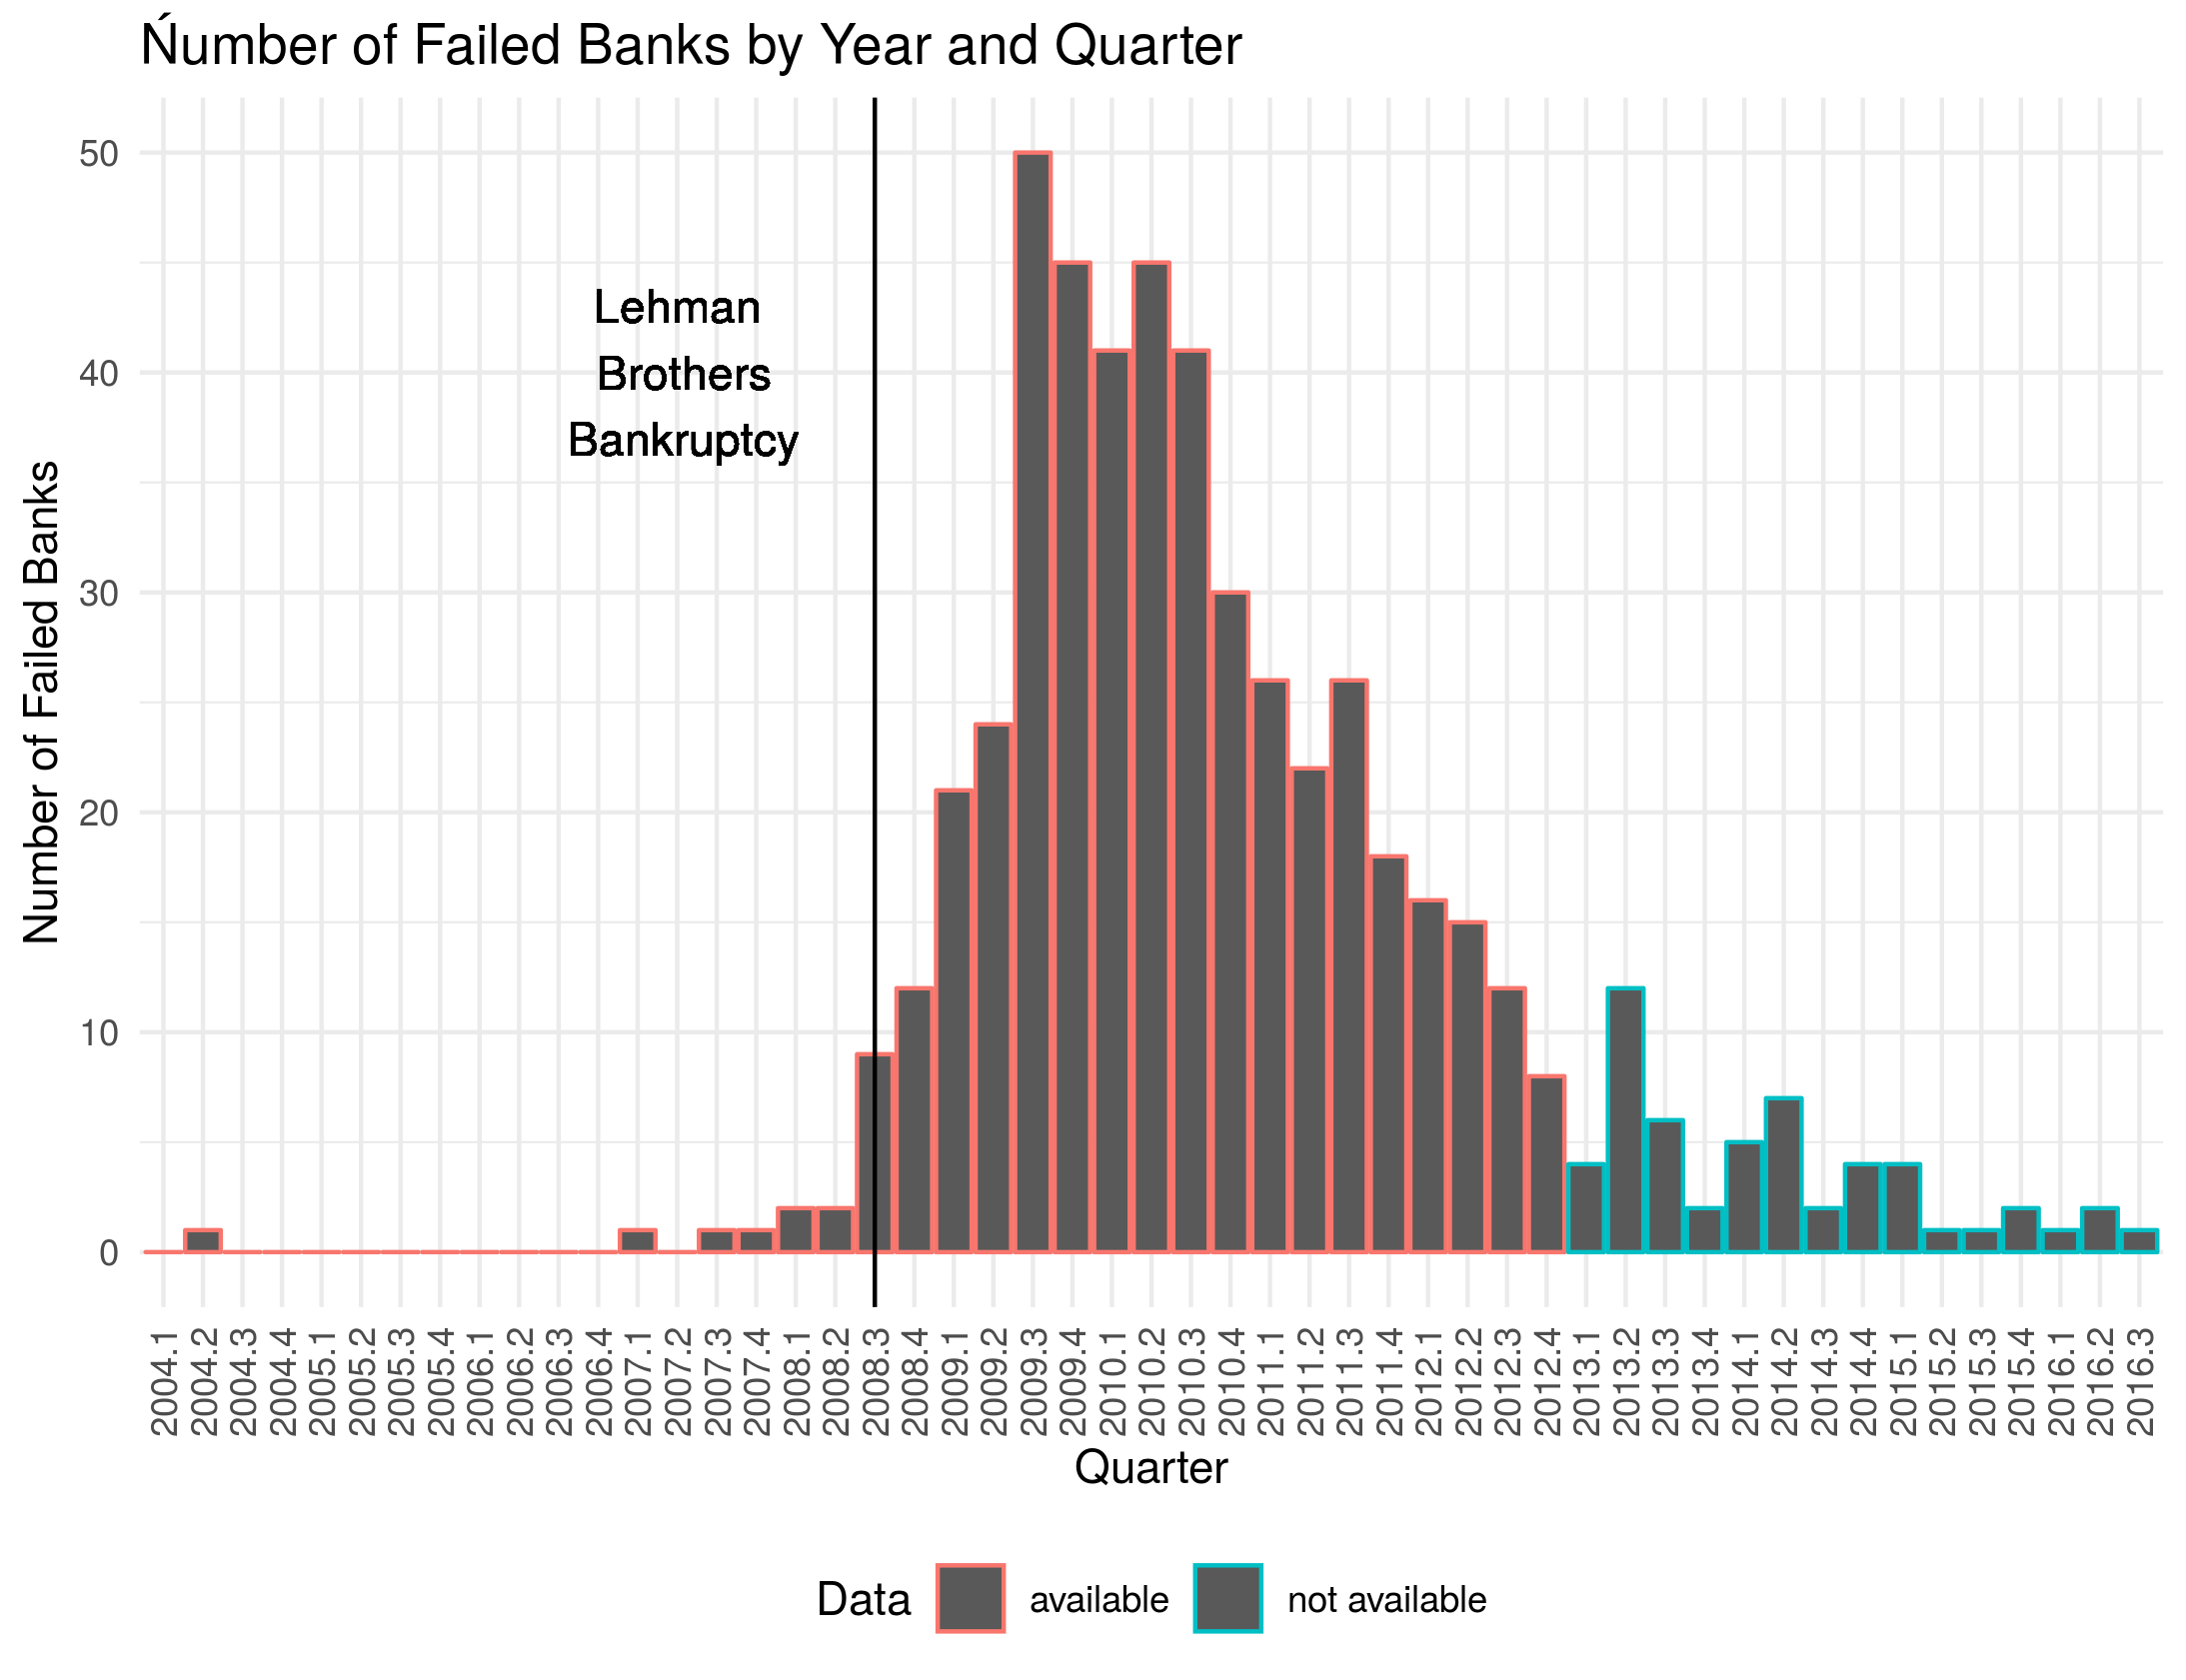
\includegraphics[width=0.9\textwidth]{failures_by_quarter_complete_with_text.png}
	\caption{Failures over all periods}
	\label{fig:failures_by_quarter}
\end{figure}
\subsection{Dataset Transformation and Preprocessing}
Before the actual training and prediction procedure can take place, several preprocessing steps have to be implemented. By contrast to the Master Thesis which served as an inspiration for this project, the feature engineering process was done in a more simple manner. Because of the fact that we're dealing with models which need to be provided with the same number of features for every observation, I fixed a number of lagged variables which should be used as inputs later on. Additionally I fixed the prediction horizon to $h=2$. The actual dataset was constructed by sliding over the dataframe with a handwritten function, returning a dataframe in wide format, where every single row or observation represents one bank at one time point $t$. 
The features were constructed by introducing the lags of each variable up to six periods in the past which leaves us with the 91 variables tabled in Table \vref{tab:lagged_dataset}, where \verb+"eq_1"+ stands for the equity of a bank in period $t-1$ and so on. The target variable \verb+"Perform_2"+ represents the Performance of the respective bank with a lead of 2 periods to account for the prediction horizon $h = 2$.
% Please add the following required packages to your document preamble:
% \usepackage{booktabs}
\begin{table}[]
\centering
\begin{tabular}{@{}ll@{}}
\toprule
\textbf{Var\#} & \textbf{Name} \\ \midrule
1              & eq\_1         \\
2              & lnatres\_1    \\
3              & roa\_1        \\
4              & sc\_1         \\
5              & bro\_1        \\
6              & log\_asset\_1 \\
7              & chbal\_1      \\
8              & intan\_1      \\
$\vdots$       & $\vdots$      \\
90             & asset\_6      \\
91             & Perform\_2    \\ \bottomrule
\end{tabular}
\caption{Dataset after introducing lagged variables}
\label{tab:lagged_dataset}
\end{table}
After this transformation for the sake of simplicity only complete cases were kept in the dataset. This obviously removes all observations, which held missing values before the transformation of the dataframe. Additionally every observation is removed where the window slides over the edge of the dataframe. This means the respective lagged variables can't be created because the respective values don't exist in the dataset or the performance variable in $t+2$ of the bank is not part of the dataset, making a prediction impossible. This holds for the last two periods in the dataset.\par
\subsubsection*{Training-Test-Split}
After the dataset is brought to the described format I went on to the usual split into a training and a validation or test set. I am assigning 80\% of the total observations to the training and 20\% of the total observations to the test set. Both in the training and the test set the class imbalance is severe if we construct the dataset in that way. Successful banks make up for 99.8\% of the total observations, while the banks failing two periods ahead in the future account for only 0.2\%. The absolute an relative numbers can be found in Table \vref{tab:ratios_train_test}.
% Please add the following required packages to your document preamble:
% \usepackage{booktabs}
\begin{table}[]
\centering
\begin{tabular}{@{}llll@{}}
\toprule
 & nonfailure & failure & $\Sigma$ \\ \midrule
Train Set Abs. & 180,344 & 380 & 180,724 \\
Rel.: & 0.9979 & 0.0021 &  \\
Test Set Abs. & 45,092 & 88 & 45,180 \\
Rel.: & 0.9981 & 0.0019 &  \\ \midrule
Complete Lagged Dataset & 225,436 & 468 & 225,904
\end{tabular}
\caption{Target Class Ratio in imblanaced Train and Test Set}
\label{tab:ratios_train_test}
\end{table}
\subsubsection*{Normalization}
Because the SMOTE algorithm implicitly uses an (euclidean) distance measure for the calculation of the nearest minority neighbors, the normalization of the observations is necessary even if we might not know yet which algorithm we want to apply. It is crucial to normalize the training and testing dataset separately, the normalization should therefore be done after the training-test split. If we would normalize before the split, we leak information from the training into the test set. That's why we save the respective preprocessing values, standard deviation and mean of the training data, and apply it to the test data afterwards:
\begin{minted}{R}
# save preProcValues for imbalanced trainSet:
preProcValues <-preProcess(trainSet_imbalanced, 
                            method = c("center","scale")) 
# scale and center train set:
trainSet_imbalanced_pre <- predict(preProcValues, trainSet_imbalanced) 
# apply same values to testSet:
testSet_pre <- predict(preProcValues, testSet)                         
\end{minted}
This leaves us with a preprocessed version of the training and the test set, which can directly serve as input and validation for a classification algorithm. As we'll see in a second there is one drawback of doing the preprocessing in a separate step in advance. When doing cross-validation, it is best practice to implement the center and scaling step right into the cv. The reason for this is the same as for preprocessing training and test set separately. Let's assume 5-fold cross-validation in our case. This means during each fold 80\% of the original training set will be used for fitting a model, while 20\% are the holdout used for validation. We shouldn't have any information leakage from the 80\% to the 20\% if we want to have an unbiased estimation, of how well the model is doing on unknown data. That's why our training procedure is actually implemented on the raw dataset and not on the preprocessed one, even if Smote is not present.

I passed on further feature engineering because of the fact that the needed input features, the CAMEL variables, were readily delivered in the dataset. So after the whole dataset has been split and normalized, we can go on to the actual training procedure.
\subsection*{Cross Validation and Hyperparameter Tuning}
This section actually is right in between preprocessing and the actual training process. Nevertheless, I shortly want to discuss how a training procedure is set up at the hand of one single example, which can be found in Appendix \vref{app:training_set_up}. During the set up of the training procedure there are 5 different objects defined, which are relevant during the optimization process. We mentioned already that we want to make use of cross validation (cv), which gives more robust measures of the generalization capabilities of the algorithm. For this the \verb+createFolds()+ function splits the training data into 5 subgroups (because $k=5$) and during each repetition of the cv one of those subsets is used as a holdout while the others are used for fitting the model. We're actually applying a 5 times repeated 5-fold cv in this case. 5-fold means that the training data set is split into 5 disjoint subsets as described. The repeated stands for the fact that each single one of those serves as a hold out exactly once.

The next object, the tuning grid, is responsible for specifying a set of hyperparameters, of which each combination is tested and evaluated during the training process. We will discuss the specific hyperparameters in the next subsection when talking about the used training algorithm. The third, the \verb+ctrl+ object is used by caret to save the options and parameters of the training procedure. This function gets passed the just specified hyperparameters and folds for example. Additionally caret offers the possibility to specify customized sampling functions, which can also be passed to the \verb+trainControl()+ function. In our case we define the list object \verb+smote_customized1+ which holds the \verb+SMOTE()+ function from the DMwR package \cite{Torgo2010}. In the function we can specify the wanted oversampling \verb+perc.under+ and undersampling rate \verb+perc.under+ and the calculated nearest neighbors \verb+k+. By setting \verb+first = FALSE+ we specify the sequence of the preprocessing and the oversampling. Because we want the oversampling to take place AFTER the preprocessing, we set this argument to false. As discussed earlier, SMOTE uses a knn algorithm, which works best on standardized data, why this could be advantageous. Unfortunately, I was not able to introduce any of the SMOTE parameters in the hyperparameter grid, which would have actually been one of the most interesting points for this project. For now we'll just do cross validation and parameter tuning of the remaining parameters for three different customized SMOTE functions defined in advance.


The defined list object is then also passed to the \verb+trainControl()+ function as an argument of the sampling option. Using this method we have the possibility to directly implement the oversampling into the cross validation process. As we know, during the cross validation we want to check how well the model generalizes, why only the subsets used for the training in each subset must be smoted, while the holdout set has to stay untouched.\par
Finally we can pass all the objects to the \verb+train()+ function, which is responsible for fitting the specified algorithm to the whole training set. It also specifies the whole training data set, the used algorithm, the preprocessing steps (scaling and centering) and the metric, which is used as the maximization criterion. Be aware again, that we used an unpreprocessed and an unbalanced version of the training set as an input because all the steps are implicitly done during the cross-validation.
\section{Technical Background: Algorithm}
The focus in this project clearly is about the influence SMOTING of the underlying imbalanced dataset has on a trained model's accuracy. It is not about the comparison of different learning algorithms. For this application I chose a \textbf{Gradient Boosting Machine} to check which influence SMOTE actually has on the learning outcome. Before I'll report the outcome of the respective implementation I want to give some very short background about the algorithm itself.
\subsection{Gradient Boosting Machine}
The approach applied to the problem, the Gradient Boosting Machine (GBM), was originally proposed by Friedman in 2001 \cite{friedman2001greedy}. GBM can be described as an ensemble technique, meaning it makes use of different weak learners (decision trees) whose combination leads to a stronger learner. The underlying weak learners could be different learning algorithms in general. As the name suggests GBM falls in the class of boosting techniques, which by contrast to bagging approaches, combine the weak learners sequentially and depending on each other. In bagging approaches, for which a Random Forest is a prominent example, several weak learners are trained on random subsamples of the training data independently from each other. In the end they are combined by a voting technique to get the final prediction for a data point \cite{aggarwalClassBook}. In boosting by contrast, we iteratively correct for errors we did in the last iteration. Each iteration therefore is dependent on the preceding iterations. In each step we put more weight on the observations which have been misclassified in the last one and such are able to improve the algorithm's overall ability to generalize step by step, while each single learner's quality in the beginner could have been close to random guessing. (ibid.)

In our case we're using the standard implementation of the caret package \cite{pack::caret}. The lookup function returns the model's parameters which we can use in a hyperparameter tuning. We'll define a set to deliver caret with a tuning grid which it should use for a systematical search for an optimal parameter combination. 
\begin{Verbatim}[fontsize=\small]
    modelLookup("gbm")
  model         parameter                   label forReg forClass probModel
1   gbm           n.trees   # Boosting Iterations   TRUE     TRUE      TRUE
2   gbm interaction.depth          Max Tree Depth   TRUE     TRUE      TRUE
3   gbm         shrinkage               Shrinkage   TRUE     TRUE      TRUE
4   gbm    n.minobsinnode Min. Terminal Node Size   TRUE     TRUE      TRUE
\end{Verbatim}
The \verb+n.trees+ parameter specifies the number of iterations or trees which are constructed one after another. Finding an optimal number of iterations can be particularly important for the prevention of overfitting. It might be the case that with a larger number of iterations, we would be able to fit the training data even better, at the expense of overfitting and decreasing quality on an independent test set. By introducing the parameter in the hyperparameter tuning and using cross validation, we can guarantee that an optimal number of trees is found, which manage to generalize well. The specified vector in the code below leads to 1500 iterations in each fold \cite{friedman2001greedy}. It should be obvious that increasing the number of trees leads to a proportionate increase in computational time.

The \verb+shrinkage+ parameter can be described as a learning rate, which is a multiplicator for every update step. Smaller shrinkage rates therefore stand for a longer training time and a slower convergence (ibid.). Friedman proposes a joint optimization of both parameters because lowering the shrinkage rate, increases the best value for M. In the example below though, the shrinkage rate is held constant at caret's standard value of 0.1. Further lowering the shrinkage parameter might bring better results, but was not an option due to the limited computational power and also time available.

The remaining parameters do specify how one single base learner is actually constructed, the \verb+interaction.depth+ and \verb+n.minobstinnode+. The further specifies the maximum depth of each tree or the possible interactions between the variables, where the default value 1 stands for a purely additive model without interaction effects, a value of 2 allows for 2-way interactions and so on \cite{Torgo2010}. The latter stands for the minimum number of observations in the terminal nodes (ibid.).  
\begin{minted}{R}
tuneGridgbm <- expand.grid(interaction.depth = c(1,2,3,5,10), 
                        n.trees = c(1,2,3,10,15,30)*50,
                        shrinkage = 0.1,
                        n.minobsinnode = 10)
\end{minted}
This model can now serve as a benchmark. As stated before, this project is not too much about finding the best model for the whole problem of banking default prediction but rather to find out how SMOTE can improve the performance of a rather simple model in a very specific setting.
\section{Results}
The rest of the paper will be used to compare four different models. Please be aware that this is by no means enough for a whole grown scientific evaluation. It should rather help to get an intuition how Smote can improve the results achieved by a Gradient Boosting Machine. It can be seen as a starting point from where you could set up a more sophisticated workflow. This especially refers to the implementation of the Smote parameter into the parameter tuning and a broader set of hyperparameters for the GBM, allowing for lower shrinkage rates should be an option as soon as more time and also computational power is at hand.

For now we'll stick to one benchmark model trained on the imbalanced dataset, by contrast to three GBM models trained on data oversampled by different variations of SMOTE. A short overview over the different model specifications and especially the different variations of the SMOTE oversampling can be found in Table \vref{tab:model_specifications}. As you can see every single model was trained with a 5-fold repeated cross validation, each optimizing over the same hyperparameter grid, where the last two parameters have kept constant. During each repetition of the cv every possible combination of the number of trees (1,2,5,50,100,150,500,750,1000,1500) and an interaction depth between 1 and 10 is evaluated and the best performing model can be extracted afterwards.
\begin{minted}{R}
tuneGridgbm <- expand.grid(interaction.depth = 1:10, 
                        n.trees = c(1,2,5,c(1,2,3,10,15,30)*50),
                        shrinkage = 0.1,
                        n.minobsinnode = 10) 
\end{minted}
Also the standardization, scaling and centering, within the cross validation is the same for every of the four models as you can see in Table \ref{tab:model_specifications}. The only significant difference and the main point we're interested in, are the different parameters of the SMOTE functions concerning their under- and oversampling rates. The \verb+perc.over+ parameter basically sets the size of the final \enquote{balanced} dataset. As you would expect, the values are given in percent, \verb+perc.over = 10,000+ therefore stands for a minority group, which is 100 times the size of the original dataset. You have to be careful about the \verb+perc.under+ parameter, which is actually a bit trick to interpret. A value of 100 percent is not meant relative to the majority dataset but means that for every minority observation (after smoting) one majority observation will be sampled from the majority group. A value of 100 for \verb+perc.under+ thus will leave you with a balanced dataset, whose size is predetermined by the oversampling rate you've chosen. In Smote Model \#3 a combination of 10,000 to 200 tells you that the majority class will be twice as big as the minority class of your target variable in the end. This is why Smote Model \#1 and \#2 are balanced by contrast to the last model.
% Please add the following required packages to your document preamble:
% \usepackage{multirow}
\begin{table}[]
\centering
\begin{tabular}{lcclll}
\hline
 & \multicolumn{1}{l}{} & \multicolumn{1}{l}{} & \multicolumn{3}{c}{SMOTE} \\ \hline
 & \multicolumn{1}{l}{Cross Validation} & \multicolumn{1}{l}{Preprocessing} & k & perc.over & perc.under \\ \hline
Model Imb. & \multirow{4}{*}{\begin{tabular}[c]{@{}c@{}}5 times rep.\\ 5-fold cv\end{tabular}} & \multirow{4}{*}{\begin{tabular}[c]{@{}c@{}}Standardize\\ with "center" and \\ "scale"\end{tabular}} & - & - & - \\
Smote Model \#1 &  &  & 5 & 4,000 & 100 \\
Smote Model \#2 &  &  & 5 & 10,000 & 100 \\
Smote Model \#3 &  &  & 5 & 10,000 & 200 \\ \hline
\end{tabular}
\caption{Overview over Model Specifications}
\label{tab:model_specifications}
\end{table} 
% Please add the following required packages to your document preamble:
% \usepackage{booktabs}

After the cross validation we can extract the best found parameters for every single model. Those can be found in Table \vref{tab:bestTunesDf}. Remember that ROC was used as a optimization metric in the cross validation so the best hyperparamters found in the tuning grid are the best regarding the model's ROC. We'll see how this best models are doing in terms of other metrics. We can see that the three more balanced models have in common that the optimal number of trees is much lower than for the model trained on the imbalanced dataset with values of 500 compared to 50 for the models trained on the smoted datasets. As we've discussed before the parameters in the last two columns were specified as constant in the tuning grid, so it's no surprise that we find a fixed value there.
\begin{table}[]
\centering
\begin{tabular}{@{}lllll@{}}
\toprule
\textbf{Dataset} & \textbf{n.trees} & \textbf{interaction.depth} & \textbf{shrinkage} & \textbf{n.minobsinnode} \\ \midrule
Imbalanced & 500 & 1 & 0.1 & 10 \\
Smote Model \#1 & 50 & 3 & 0.1 & 10 \\
Smote Model \#2 & 50 & 4 & 0.1 & 10 \\
Smote Model \#3 & 50 & 4 & 0.1 & 10 \\ \bottomrule
\end{tabular}
\caption{Best Combination of n.trees and  interaction.depth. Results from cross validation. shrinkage and n.minobsinnode kept constant.}
\label{tab:bestTunesDf}
\end{table}
\subsection{Confusion Matrices and Related Measures}
We're very interested about how our models are doing in terms of their confusion matrices and the related metrics as Accuracy, Sensitivity, Recall, Precision or the F1 score. The confusion matrices of the four models can be found in Table \vref{tab:confMat_imbalanced} to \vref{tab:confMat_smote3}. All confusion matrices are evaluated on the 20\% separated as validation or test set to guarantee a comparable result. Let's start with the benchmark model trained on the imbalanced dataset. If we have look at Table \ref{tab:confMat_imbalanced}, we can see that the model is basically useless. One single Failure observation gets classified correctly, while every other observation is just classified as a nonfailing Bank. This corresponds very well with the resulting metrics shown in Table \vref{tab:metrics}. In the first part of this paper we've talked about the fact that the vanilla accuracy is not an adequate measure in the cases of severely imbalanced datasets. The \enquote{imbalanced} model exhibits an accuracy of near to 100\% while the Recall drops close to 0. The latter gives us a much more reliable intuition about the quality of our model, representing the share of all true positives over the sum of all true positives and all false negatives. 
%%%%confusion matrix imbalanced:
% Please add the following required packages to your document preamble:
% \usepackage{multirow}
\begin{table}[]
\centering
\begin{tabular}{ccccc}
\multicolumn{2}{c}{} & \multicolumn{2}{c}{\textbf{Real Class}} &  \\
\multicolumn{2}{c}{} & \textbf{Nonfailure} & \textbf{Failure} & \textbf{$\Sigma$} \\ \cline{3-4}
\multirow{2}{*}{\textbf{Prediction}} & \multicolumn{1}{c|}{\textbf{Nonfailure}} & \multicolumn{1}{c|}{45,098} & \multicolumn{1}{c|}{81} & 45,179 \\ \cline{3-4}
 & \multicolumn{1}{c|}{\textbf{Failure}} & \multicolumn{1}{c|}{0} & \multicolumn{1}{c|}{1} & 1 \\ \cline{3-4}
 & \textbf{$\Sigma$} & 45,098 & 82 & 45180
\end{tabular}
\caption{Confusion Matrix for Imbalanced Model; Evaluated on Test Dataset}
\label{tab:confMat_imbalanced}
\end{table}
Coming back to the confusion matrices for the models trained on the Smoted datasets, we can observe that the oversampling of the training dataset actually pays off. Let's recall the parameters of the three models. The first two both are balanced but the second one is trained on more than the double amount of observations. They're both doing comparably well looking at the predictions of Failing Banks, which is our main focus. Model \#2 has a slight advantage in the \enquote{Nonfailure} column and manages to put more weight on the main diagonal of the matrix. This is also reflected by the metrics in Table \ref{tab:metrics}. The recall for both models is equally high, while the precision and specificity is slightly higher in the third model going hand in hand with a higher F1 score.
% Please add the following required packages to your document preamble:
% \usepackage{multirow}
\begin{table}[]
\centering
\begin{tabular}{ccccc}
\multicolumn{2}{c}{} & \multicolumn{2}{c}{\textbf{Real Class}} &  \\
\multicolumn{2}{c}{} & \textbf{Nonfailure} & \textbf{Failure} & \textbf{$\Sigma$} \\ \cline{3-4}
\multirow{2}{*}{\textbf{Prediction}} & \multicolumn{1}{c|}{\textbf{Nonfailure}} & \multicolumn{1}{c|}{42,206} & \multicolumn{1}{c|}{10} & 42,216 \\ \cline{3-4}
 & \multicolumn{1}{c|}{\textbf{Failure}} & \multicolumn{1}{c|}{2,892} & \multicolumn{1}{c|}{72} & 2,964 \\ \cline{3-4}
 & \textbf{$\Sigma$} & 45,098 & 86 & 45,180
\end{tabular}
\caption{Confusion Matrix for Smote Mode \#1; Evaluated on Test Dataset}
\label{tab:confMat_smote1}
\end{table}

For the confusion matrix of the third smoted model in Table \ref{tab:confMat_smote3} we can observe that the recall is going down again while the specificity is going up. This is quite intuitive: on the one hand we're still strongly oversampling the minority class but at the same time keep the nonfailing banks in the majority, even if it's only by a ratio of 2:1. This is confirmed by the metrics in Table \ref{tab:metrics}.  The recall is going down to 87\% while the specificity is going up by around 1.5 percentage points to 96.05\%. We should always keep in mind this trade off between different measures, when applying oversampling techniques, having our original intention in mind. In the context of banking failures you could argue, you want a model which gives you a broader estimation with a high recall at cost of some percentage points in specificity. This results in a lot of false positive, which need a closer look but at least you can be confident that you got a lot of the problematic banks covered with your prediction.
%%%confusion matrix smote 2:
% Please add the following required packages to your document preamble:
% \usepackage{multirow}
\begin{table}[]
\centering
\begin{tabular}{ccccc}
\multicolumn{2}{c}{} & \multicolumn{2}{c}{\textbf{Real Class}} &  \\
\multicolumn{2}{c}{} & \textbf{Nonfailure} & \textbf{Failure} & \textbf{$\Sigma$} \\ \cline{3-4}
\multirow{2}{*}{\textbf{Prediction}} & \multicolumn{1}{c|}{\textbf{Nonfailure}} & \multicolumn{1}{c|}{42,511} & \multicolumn{1}{c|}{11} & 42,522 \\ \cline{3-4}
 & \multicolumn{1}{c|}{\textbf{Failure}} & \multicolumn{1}{c|}{2,587} & \multicolumn{1}{c|}{71} & 2,658 \\ \cline{3-4}
 & \textbf{$\Sigma$} & 45,098 & 82 & 45,180
\end{tabular}
\caption{Confusion Matrix for Smote Mode \#2; Evaluated on Test Dataset}
\label{tab:confMat_smote2}
\end{table}
%%%
%%%confusion matrix smote 3:
\begin{table}[]
\centering
\begin{tabular}{ccccc}
\multicolumn{2}{c}{} & \multicolumn{2}{c}{\textbf{Real Class}} &  \\
\multicolumn{2}{c}{} & \textbf{Nonfailure} & \textbf{Failure} & \textbf{$\Sigma$} \\ \cline{3-4}
\multirow{2}{*}{\textbf{Prediction}} & \multicolumn{1}{c|}{\textbf{Nonfailure}} & \multicolumn{1}{c|}{43,271} & \multicolumn{1}{c|}{16} & 42,522 \\ \cline{3-4}
 & \multicolumn{1}{c|}{\textbf{Failure}} & \multicolumn{1}{c|}{1,827} & \multicolumn{1}{c|}{66} & 2,658 \\ \cline{3-4}
 & \textbf{$\Sigma$} & 45,098 & 82 & 45,180
\end{tabular}
\caption{Confusion Matrix for Smote Mode \#3; Evaluated on Test Dataset}
\label{tab:confMat_smote3}
\end{table}
% Please add the following required packages to your document preamble:
% \usepackage{booktabs}
% \usepackage{graphicx}
\begin{table}[]
\centering
\resizebox{\textwidth}{!}{%
\begin{tabular}{@{}llllll@{}}
\toprule
\textbf{Dataset} & \textbf{Accuracy} & \textbf{Specificity} & \textbf{Precision} & \textbf{Recall} & \textbf{F1} \\ \midrule
Imbalanced & 0.9981 & 1 & 1 & 0.0116 & 0.023 \\
Smote Model \#1 & 0.937  & 0.937 & 0.0271 & 0.9186 & 0.0526 \\
Smote Model \#2 & 0.9436  & 0.9437 & 0.0302 & 0.9186 & 0.0584 \\
Smote Model \#3 & 0.9604  & 0.9605 & 0.0405 & 0.8721 & 0.0773 \\ \bottomrule
\end{tabular}%
}
\caption{Metrics for the models trained on the four different datasets.}
\label{tab:metrics}
\end{table}
\subsection{Graphical Analysis Cross Validation}
When talking about the metrics ROC, sensitivity, specificity and recall we can also check, how the measures develop in the cross validation by checking the graphical outputs, which caret is providing along with a train object. Those can be found in the Appendices \vref{app:cv_graphics_roc} to \vref{app:cv_graphics_spec}. In Appendix  \ref{app:cv_graphics_roc} we can see that the first graphic, the imbalanced model, is different from the last three in their basic structure. In the smoted models it seems that the ROC measure is rather stable over different Maximum Tree Depths, at least for higher numbers of boosting iterations, and is only varying over the number of iterations. The graphics confirm the best tuning parameters discussed above, the maximum is reached at lower tree depths of 3 or 4 and a number of trees of 50. We know that the first model is basically useless, so interpreting its graphic does not make any sense here, we'll rather go on to the other evaluated measures, which give some more interesting insights.

If we look at the smoted model we can see that there is basically a reversed shape of the recall (or sensitivity) on page \vref{app:cv_graphics_sens} and the specificity curves on page \vref{app:cv_graphics_spec}. With a growing tree depth the recall tends to grow, while the specificity is declining. We can assume, that if we had chosen the recall as an optimization measure during the cross validation, even higher values could have been obtained as the ones reached by our models. We can expect that the values in the graphics are quite robust because they're averaged over the different folds and repeats of the cross validation.
\subsection{Variable Importance}
What remains is a short but quite surprising look at the Variable Importance which Caret returns. Those can be found in Appendix \ref{app:variable_importance}. I've plotted the 15 variables with the most predictive power, which is more than enough because as you can see that in each of the models the scaled variable importance tends towards 0 quite fast. 

It might be caused by the short prediction horizon or the transformation of the dataset, with only the 6 last lagged periods included, but it seems that the vast majority of the predictive power of the smoted Datasets actually can be attributed to one single variable: the Return on Assets in the preceding period (\verb+roa_1+), followed by the return on assets in the period before. On the following places the Brokered deposits (\verb+bro+) of the last few periods, do seem to have some impact, which is close to or below 5\% though, when scaled to the importance of \verb+roa_1+.
\section{Conclusion}
The existence of balanced target classes often rather is a textbook scenario than a real world case. There the opposite might rather describe the normal and also most interesting applications. Usually a small fraction of the target group of a marketing campaign will actually act and buy your commodity or sign a contract, a small share of produced technical products will break after production, or as we know, a tiny amount of banks will fail at some point in the near future - all cases of highly imbalanced datasets in terms of their target variable. We've seen that this can be quite problematic and challenging, especially if you don't adapt your machine learning techniques and metrics to such a scenario. 

One important aspect of this adaption is to choose the right evaluation measures for such a model's outcome. The simple and plain accuracy, for whose optimization we often strive, is not adequate at all to measure a model's performance as we've seen when comparing the four different implemented model variations. We have to aim for other metrics and, depending what we actually prioritize, rather go for a high sensitivity/recall or precision. I would say that in the described cases, the recall often might be the measure of interest because an error in the underrepresented minority class might have severe consequences.

We got a little insight that Smote, as simple as the idea actually is, might offer a solution to such problems. Even the quite arbitrary choice of three different Smote variations delivered much better results than the benchmark trained on the imbalanced dataset. We were able to drastically improve the recall and precision of the model's turning a useless model in actually a quite promising one. This was done without any changes in the model specification but only by oversampling the underlying dataset. I want to maintain, that it is crucial to always have in mind, what our model should actually be used for and in which cases you are actually interested in. Weighing up the costs of misclassifying a positive or negative observation is very important when tackling a machine learning problem in general and one in an imbalanced scenario in particular.

The paper obviously rather is a small technical report than actually examining the area of banking default prediction. Developing (much more complex) models, which can actually help to predict failures of banks and other financial institutes might be one of the key instruments to be better prepared, when the next financial crisis hits. It would be quite interesting to dig deeper into the direction of variable importance. Having only a very little number of variables holding almost all predictive power, is quite surprising and should be thoroughly investigated.

Finally I have to note that this project does not serve as a scientific contribution at all but rather dealt as a starting point to get familiar with and get an intuition for oversampling techniques and the handling of imbalanced class distributions. There are a lot of (technical) issues which have to be resolved before such a study could provide clear insights. The most serious one is probably that the parameters of the SMOTE Function should be introduced into the hyperparameter tuning, when more time and computational power is available. Additionally a wider range should have been allowed for the \verb+perc.under+ and \verb+perc.over+ parameters. It would also be crucial to keep the \verb+k+ parameter variable and not constant (at $k=5$ as I did). Apart from the SMOTE function the same holds for the GBM model, where the Terminal Node Size should be introduced into the hyperparameter tuning. Above the step size or \verb+shrinkage+ should be lowered when a Computing Cluster is available. It is to expected that the computational time would grow by a factor of 10 if the shrinkage is lowered from $0.1$ to $0.01$, which would probably increase the quality of the model though. 
\pagebreak
\clearpage
\bibliography{library} 
\bibliographystyle{apalikelasse}
\clearpage
\pagebreak
\listoffigures
\clearpage
\pagebreak
\listoftables
\pagebreak
\addtocontents{toc}{\protect\newpage}
\begin{appendices}
\section{Exemplary Training Set Up}\label{app:training_set_up}
\begin{minted}{R}
myFolds_customSmote <- createFolds(trainSet_imbalanced_pre$Perform_2, 
                                    k = 5)
tuneGridgbm <- expand.grid(interaction.depth = 1:10, 
                           n.trees = c(1,2,5,c(1,2,3,10,15,30)*50),
                           shrinkage = 0.1,
                           n.minobsinnode = 10)

smote_customized1 <- list(name = "SMOTE with more neighbors!",
                func = function (x, y) {
                  library(DMwR)
                  dat <- if (is.data.frame(x)) x else as.data.frame(x)
                  dat$.y <- y
                  dat <- SMOTE(.y ~ ., data = dat, perc.over = 4000, 
                  perc.under = 100, k = 5)
                  list(x = dat[, !grepl(".y", colnames(dat), 
                  fixed = TRUE)], 
                       y = dat$.y)
                },
                first = FALSE) 

ctrl <- trainControl(method = "repeatedcv", repeats = 5,
                     classProbs = TRUE,
                     verboseIter = TRUE,
                     savePredictions = TRUE,
                     index = myFolds_customSmote, #pass folds from above 
                     summaryFunction = twoClassSummary,
                     sampling = smote_customized1) 
#fit model to training set:
smote_model_customized1 <- train(Perform_2 ~ ., data = trainSet_imbalanced, 
      method = "gbm",
      trControl = ctrl,
      preProcess=c("scale", "center"),
      tuneGrid = tuneGridgbm,
      metric = "ROC",
      maximize = TRUE)
\end{minted}
\section{Cross Validation Graphics - ROC}\label{app:cv_graphics_roc}
\begin{figure}[h!] % "[t!]" placement specifier just for this example
\begin{subfigure}{0.48\textwidth}
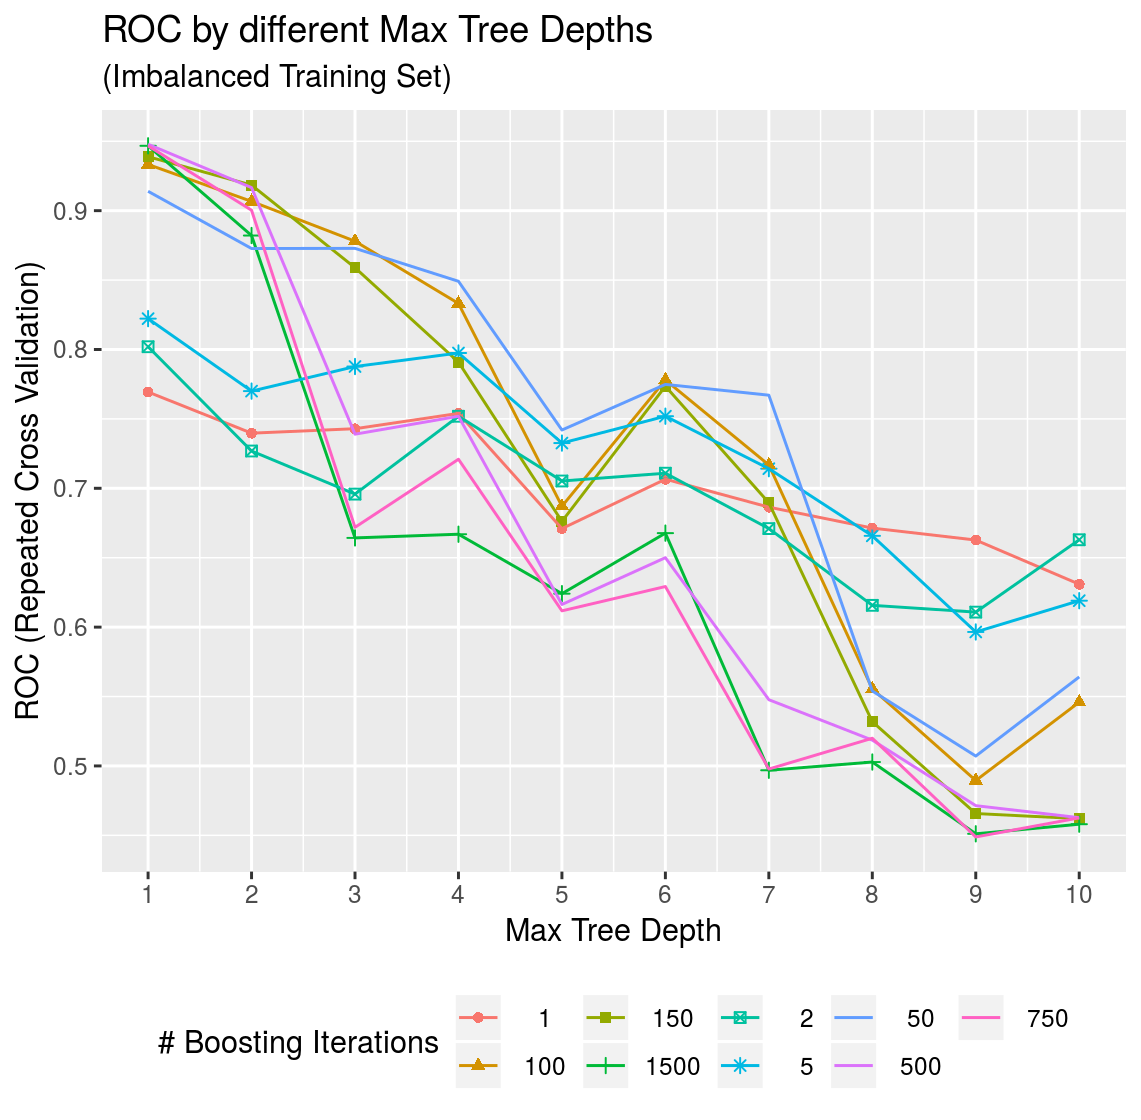
\includegraphics[width=\linewidth]{./graphics/cv/ROC_by_treeDepth_complete.png}
\caption{Imbalanced Model} \label{app:cv_graphics_roc_imb}
\end{subfigure}\hspace*{\fill}
\begin{subfigure}{0.48\textwidth}
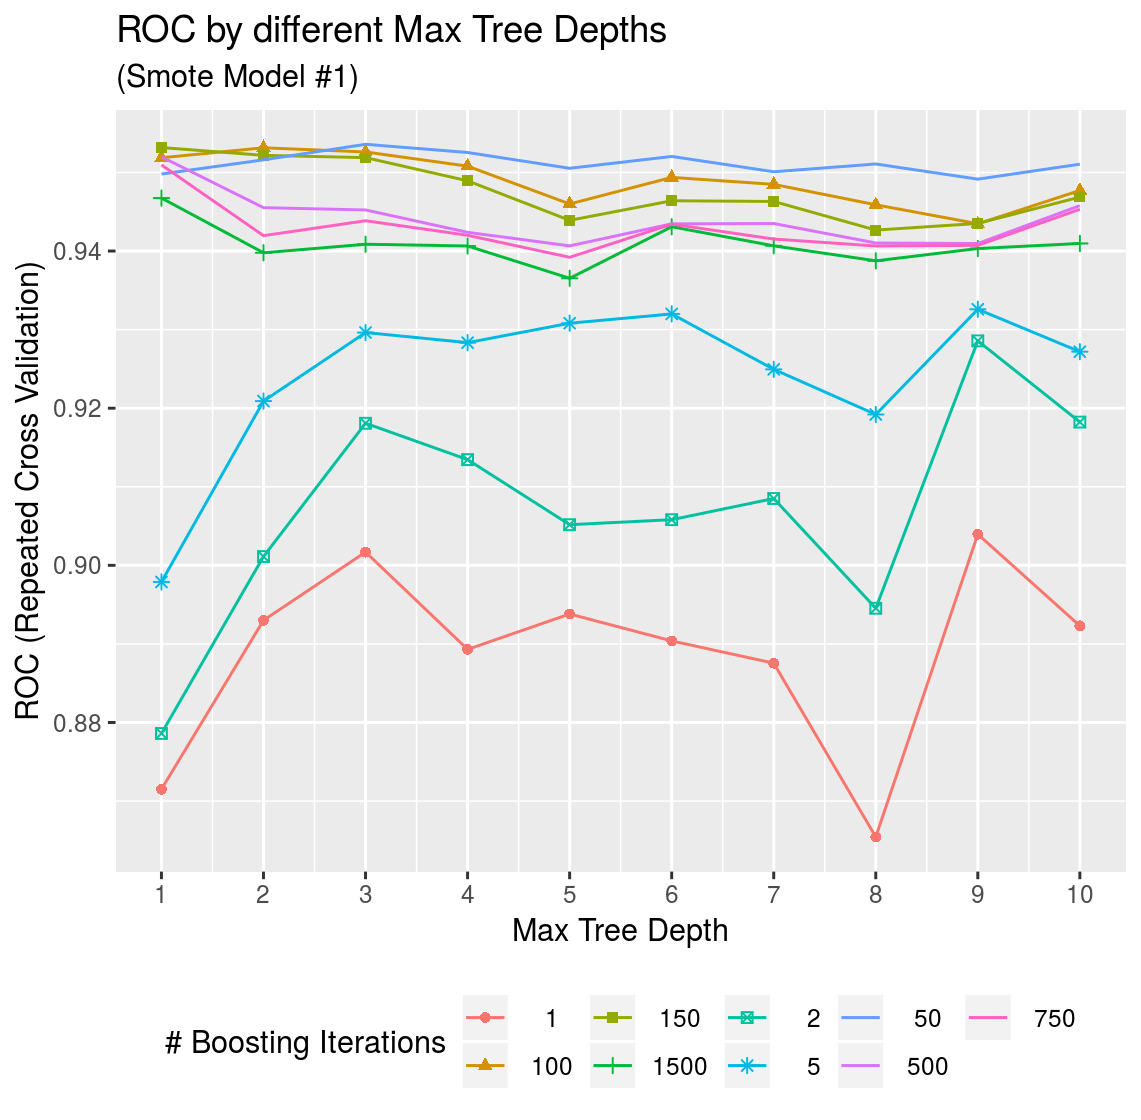
\includegraphics[width=\linewidth]{./graphics/cv/ROC_by_treeDepth_smote1.png}
\caption{Smote Model \#1} \label{app:cv_graphics_roc_smote1}
\end{subfigure}
\begin{subfigure}{0.48\textwidth}
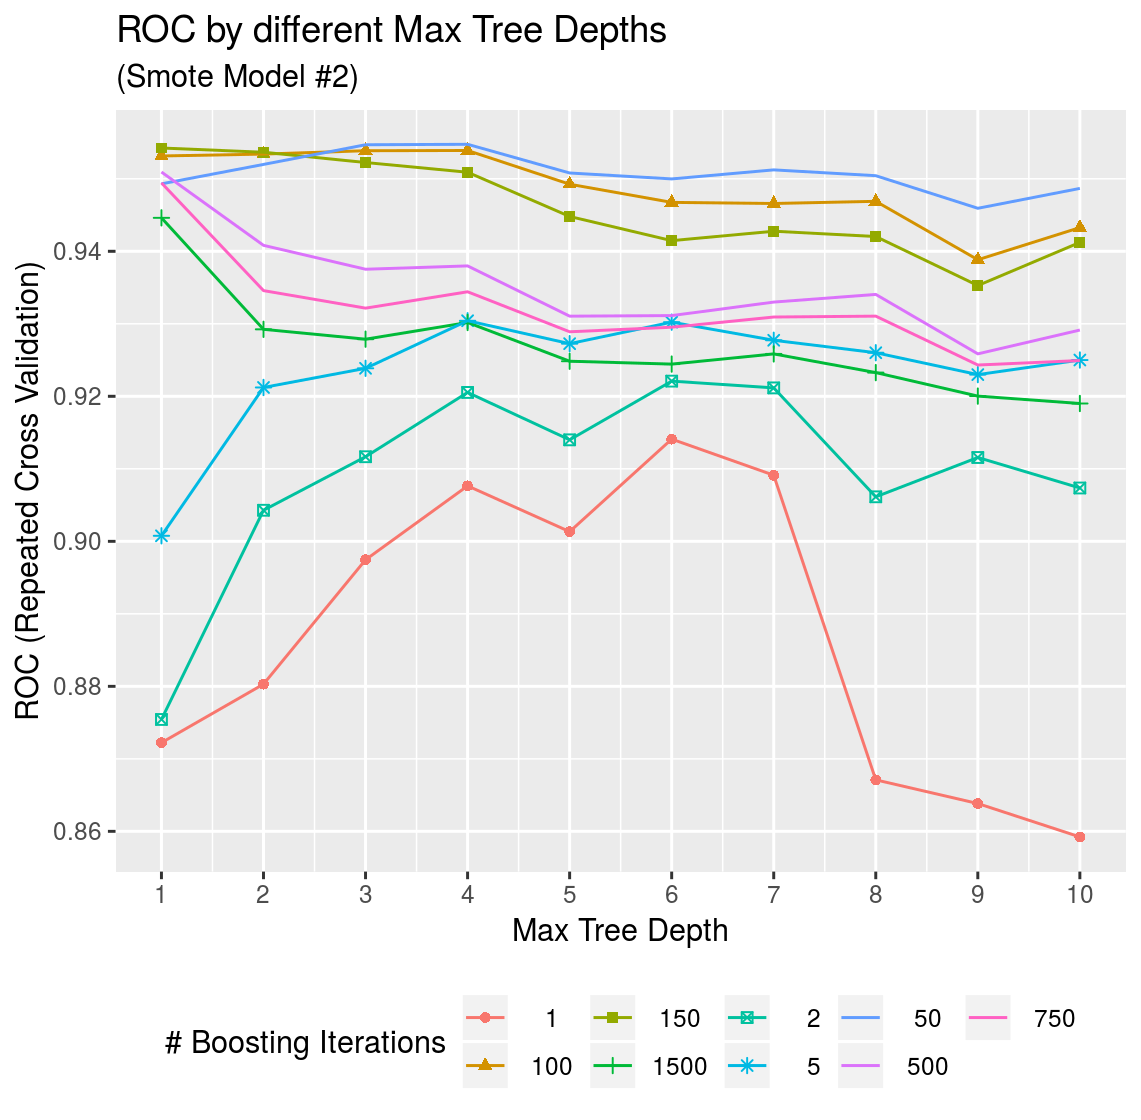
\includegraphics[width=\linewidth]{./graphics/cv/ROC_by_treeDepth_smote2.png}
\caption{Smote Model \#2} \label{app:cv_graphics_roc_smote2}
\end{subfigure}\hspace*{\fill}
\begin{subfigure}{0.48\textwidth}
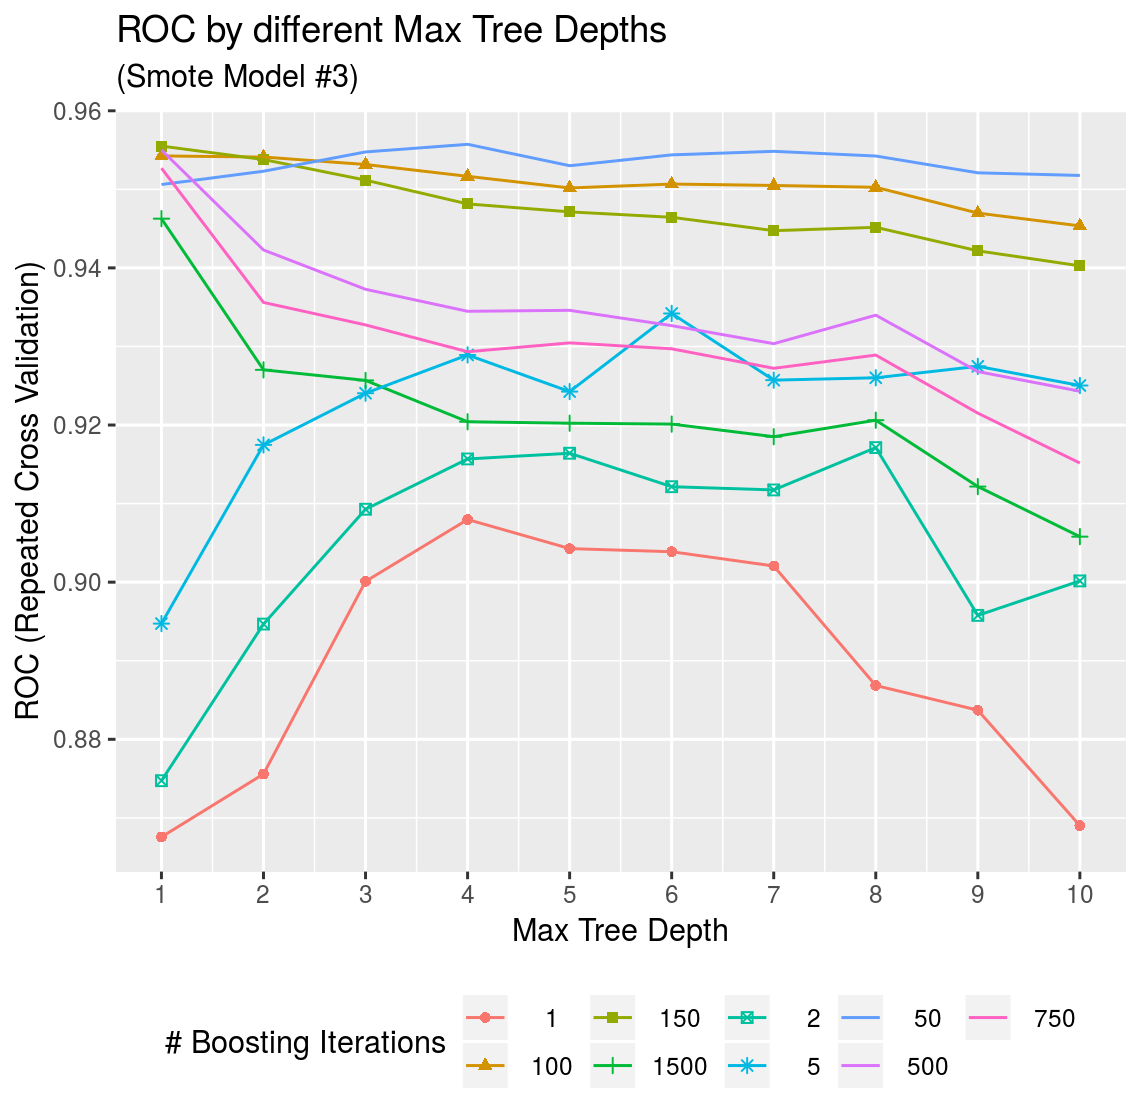
\includegraphics[width=\linewidth]{./graphics/cv/ROC_by_treeDepth_smote3.png}
\caption{Smote Model \#3} \label{app:cv_graphics_roc_smote3}
\end{subfigure}
\caption{Cross Validation: ROC by Max Tree Depth and Number of Iterations} \label{fig:2}
\end{figure}
\pagebreak\clearpage
\section{Cross Validation Graphics - Sensitivity}\label{app:cv_graphics_sens}
\begin{figure}[h!] % "[t!]" placement specifier just for this example
\begin{subfigure}{0.48\textwidth}
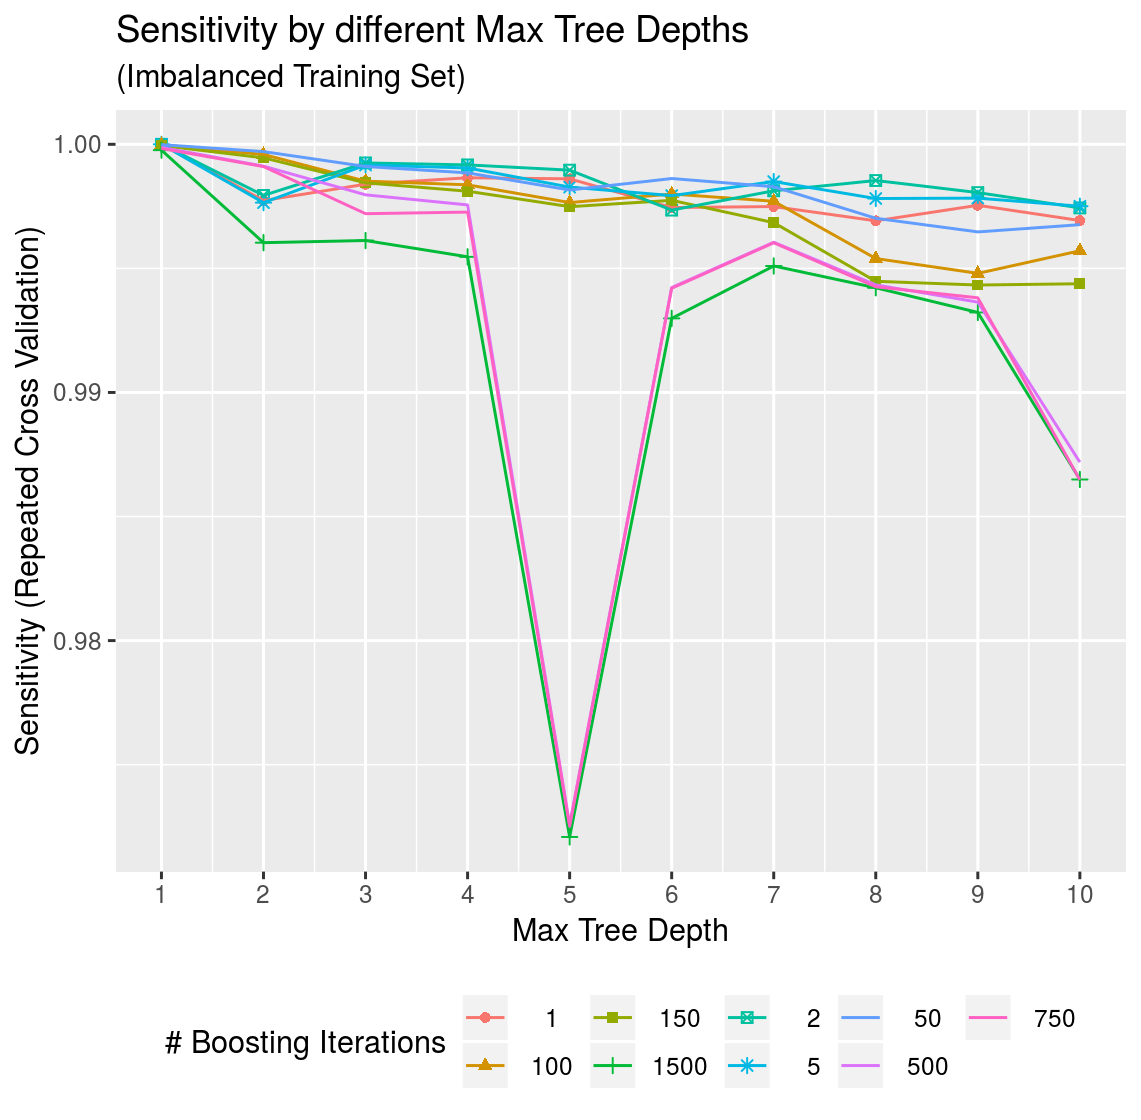
\includegraphics[width=\linewidth]{./graphics/cv/Sens_by_treeDepth_complete.png}
\caption{Imbalanced Model} \label{fig:a}
\end{subfigure}\hspace*{\fill}
\begin{subfigure}{0.48\textwidth}
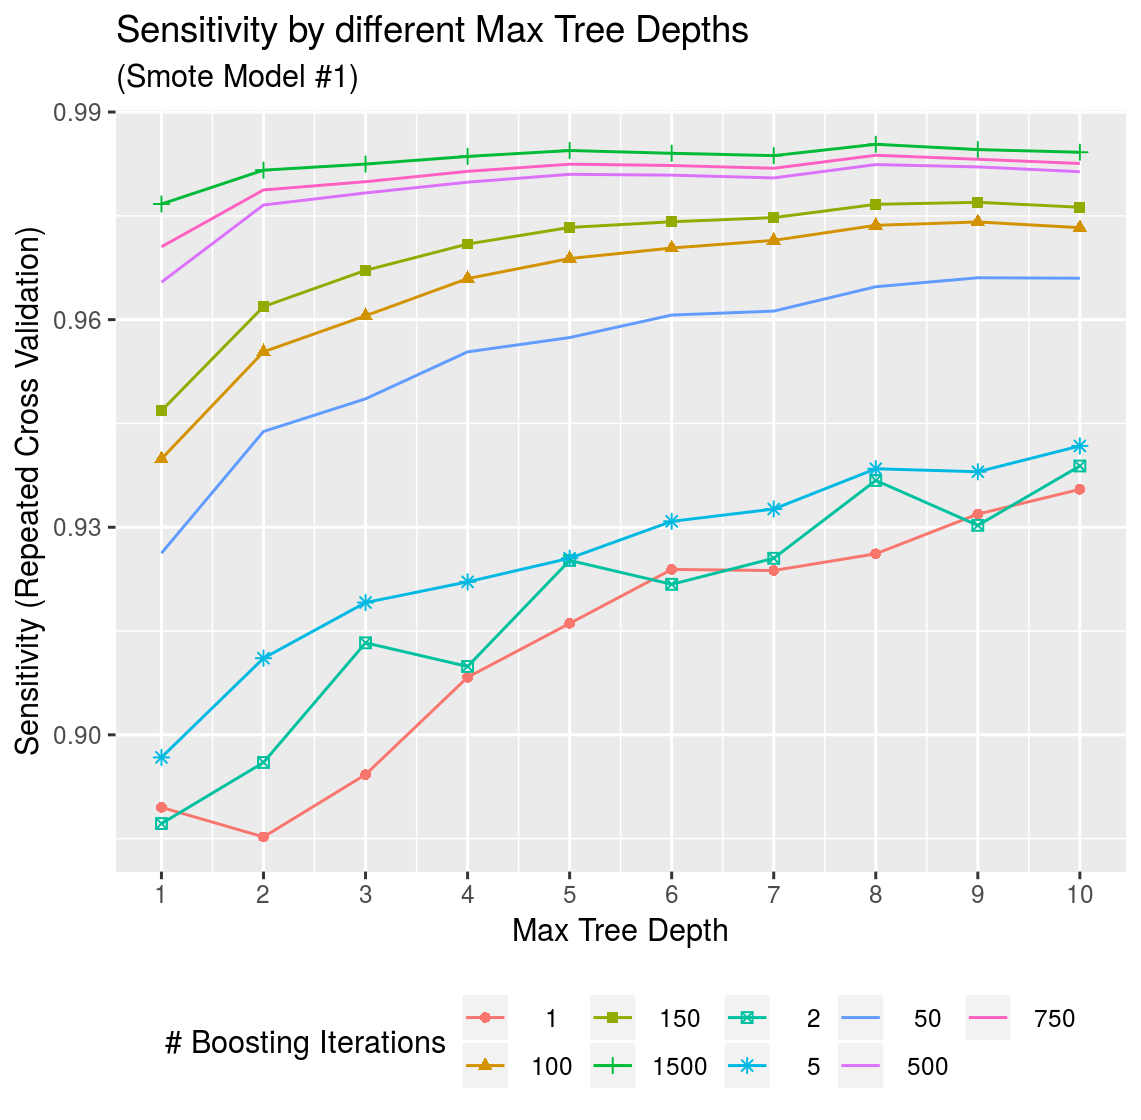
\includegraphics[width=\linewidth]{./graphics/cv/Sens_by_treeDepth_smote1.png}
\caption{Smote Model \#1} \label{fig:a}
\end{subfigure}
\begin{subfigure}{0.48\textwidth}
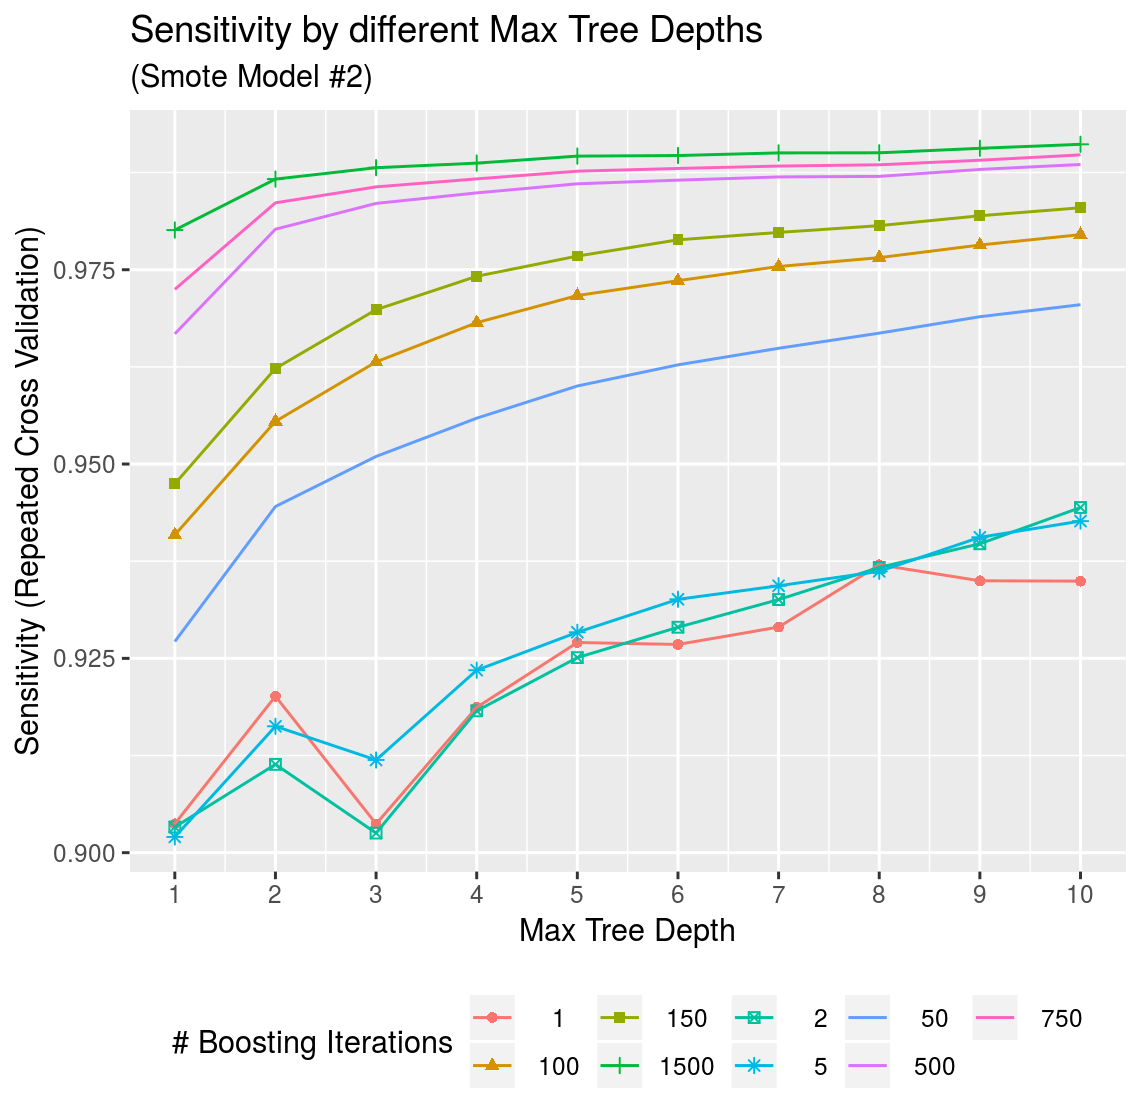
\includegraphics[width=\linewidth]{./graphics/cv/Sens_by_treeDepth_smote2.png}
\caption{Smote Model \#2} \label{fig:a}
\end{subfigure}\hspace*{\fill}
\begin{subfigure}{0.48\textwidth}
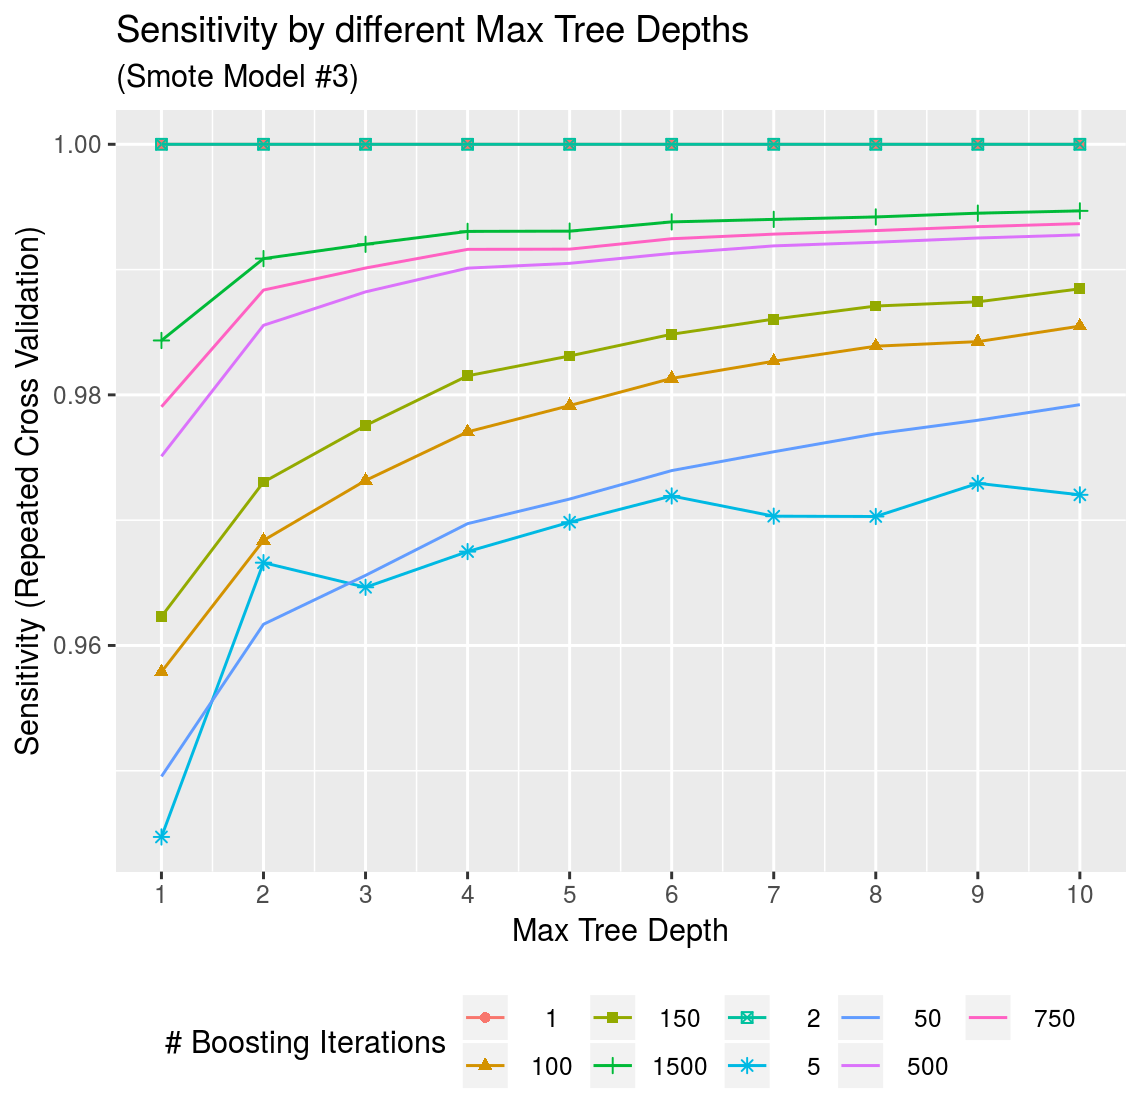
\includegraphics[width=\linewidth]{./graphics/cv/Sens_by_treeDepth_smote3.png}
\caption{Smote Model \#3} \label{fig:a}
\end{subfigure}
\caption{Cross Validation: Sensivity by Max Tree Depth and Number of Iterations}
\end{figure}
\pagebreak
\clearpage
\section{Cross Validation Graphics - Specifity}\label{app:cv_graphics_spec}
\begin{figure}[h!] % "[t!]" placement specifier just for this example
\begin{subfigure}{0.48\textwidth}
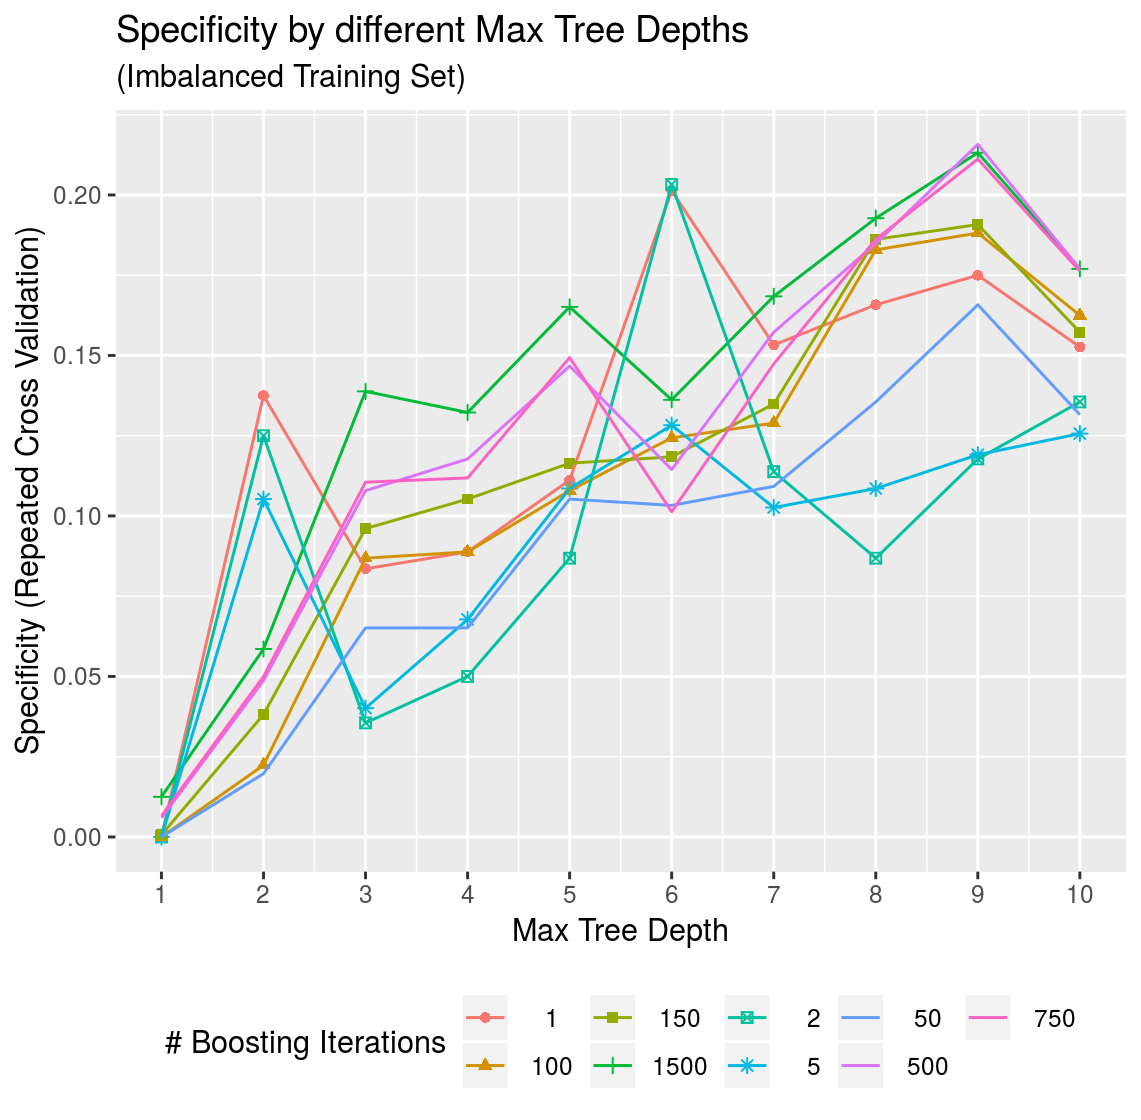
\includegraphics[width=\linewidth]{./graphics/cv/Spec_by_treeDepth_complete.png}
\caption{Imbalanced Model} \label{fig:a}
\end{subfigure}\hspace*{\fill}
\begin{subfigure}{0.48\textwidth}
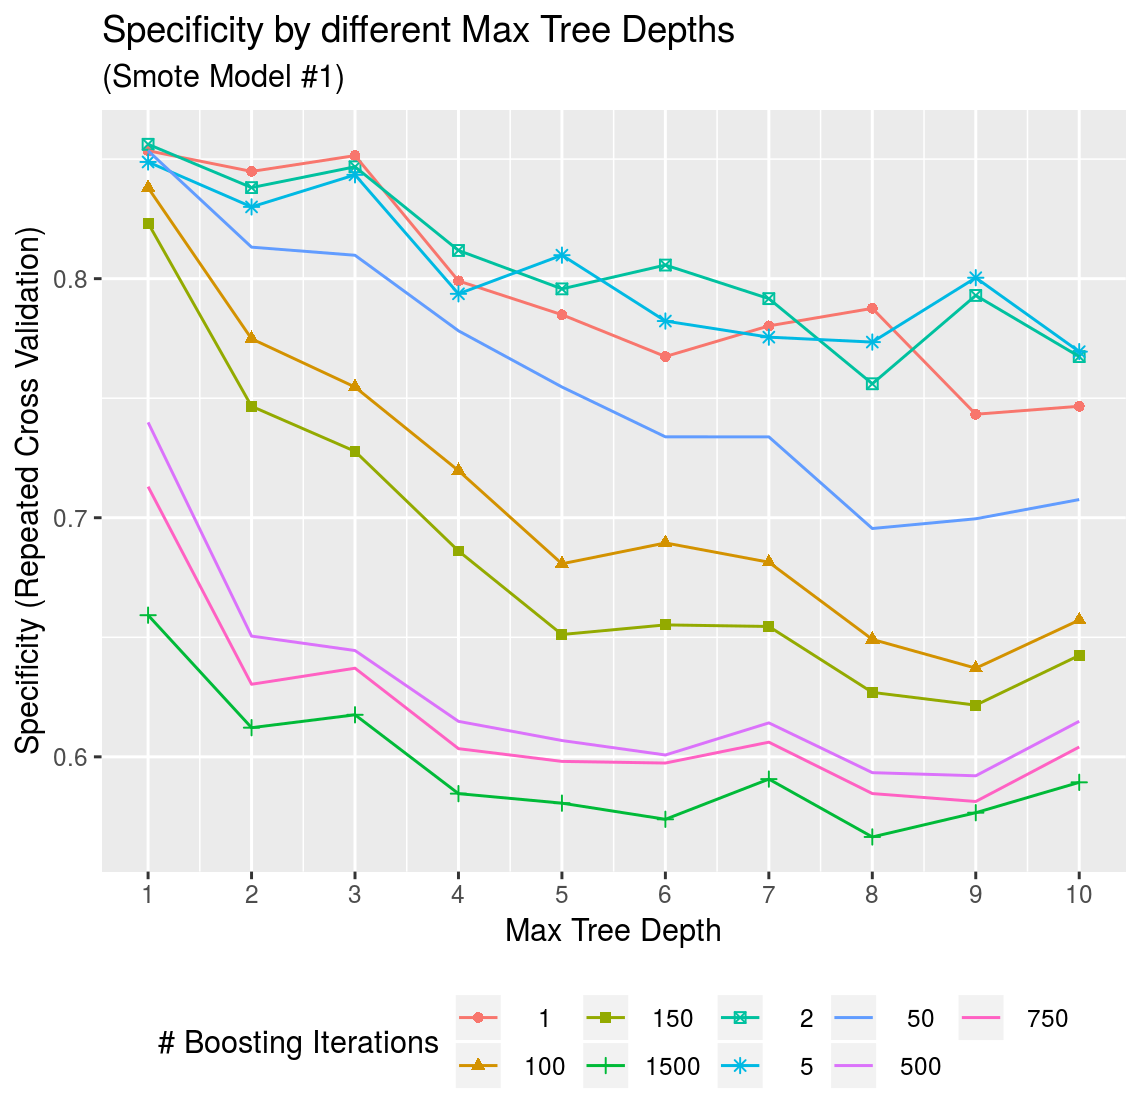
\includegraphics[width=\linewidth]{./graphics/cv/Spec_by_treeDepth_smote1.png}
\caption{Smote Model \#1} \label{fig:a}
\end{subfigure}
\begin{subfigure}{0.48\textwidth}
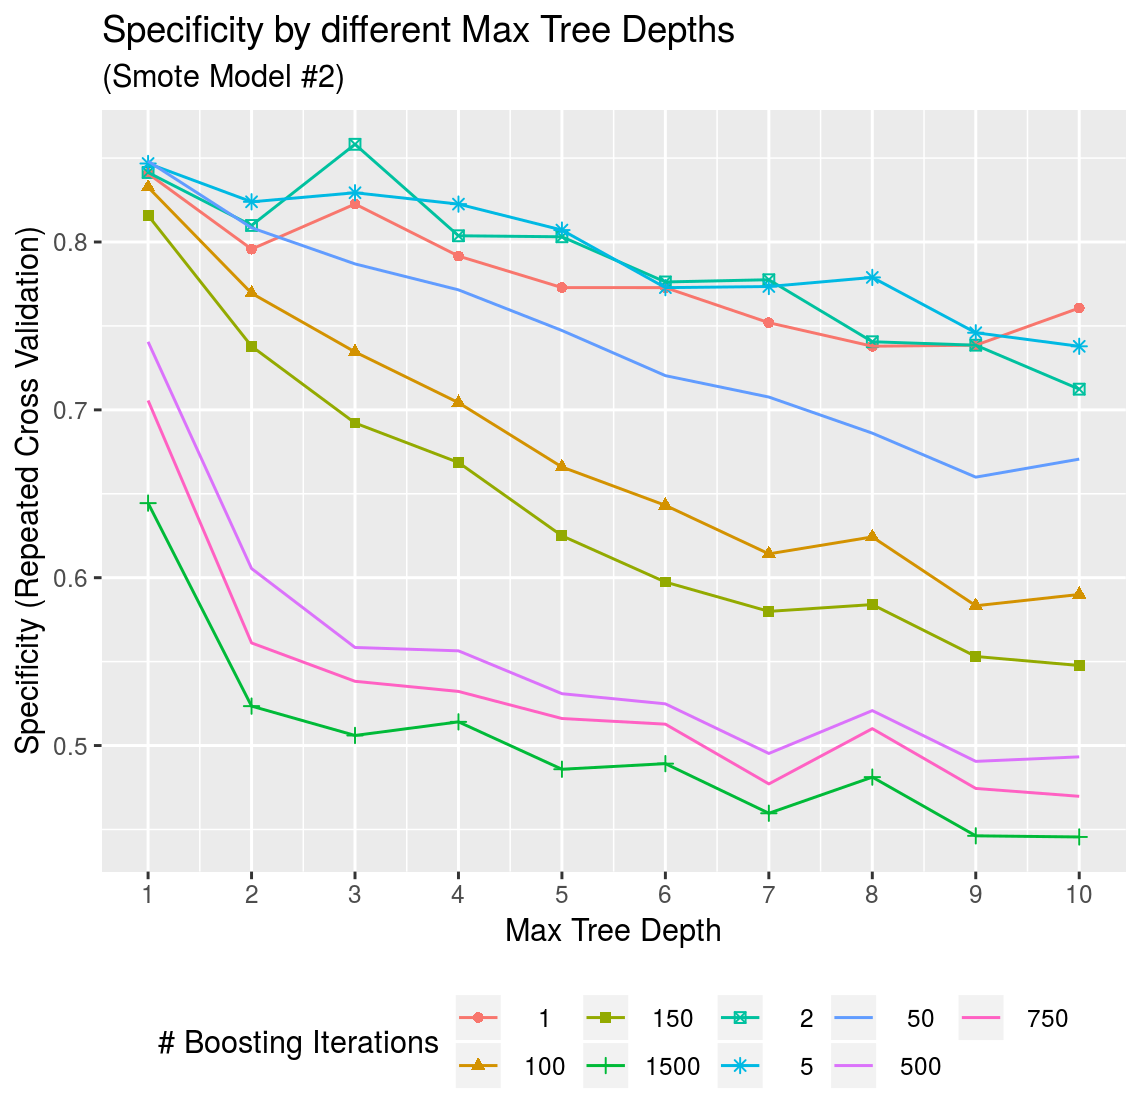
\includegraphics[width=\linewidth]{./graphics/cv/Spec_by_treeDepth_smote2.png}
\caption{Smote Model \#2} \label{fig:a}
\end{subfigure}\hspace*{\fill}
\begin{subfigure}{0.48\textwidth}
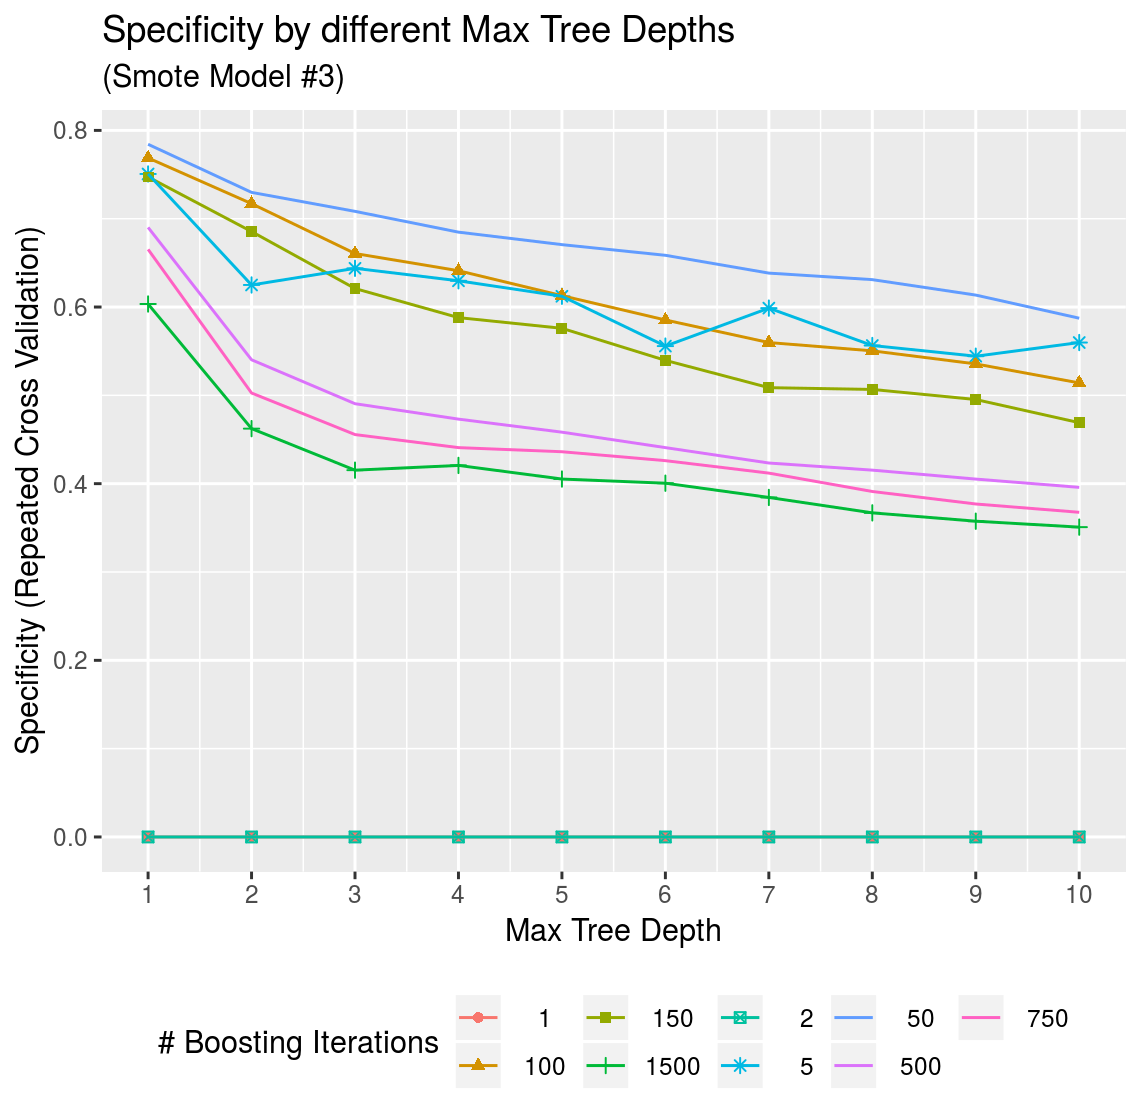
\includegraphics[width=\linewidth]{./graphics/cv/Spec_by_treeDepth_smote3.png}
\caption{Smote Model \#3} \label{fig:a}
\end{subfigure}
\caption{Cross Validation: Specifity by Max Tree Depth and Number of Iterations}
\end{figure}
\pagebreak
\clearpage
\section{Variable Importance}\label{app:variable_importance}
\begin{figure}[h!] % "[t!]" placement specifier just for this example
\begin{subfigure}{0.48\textwidth}
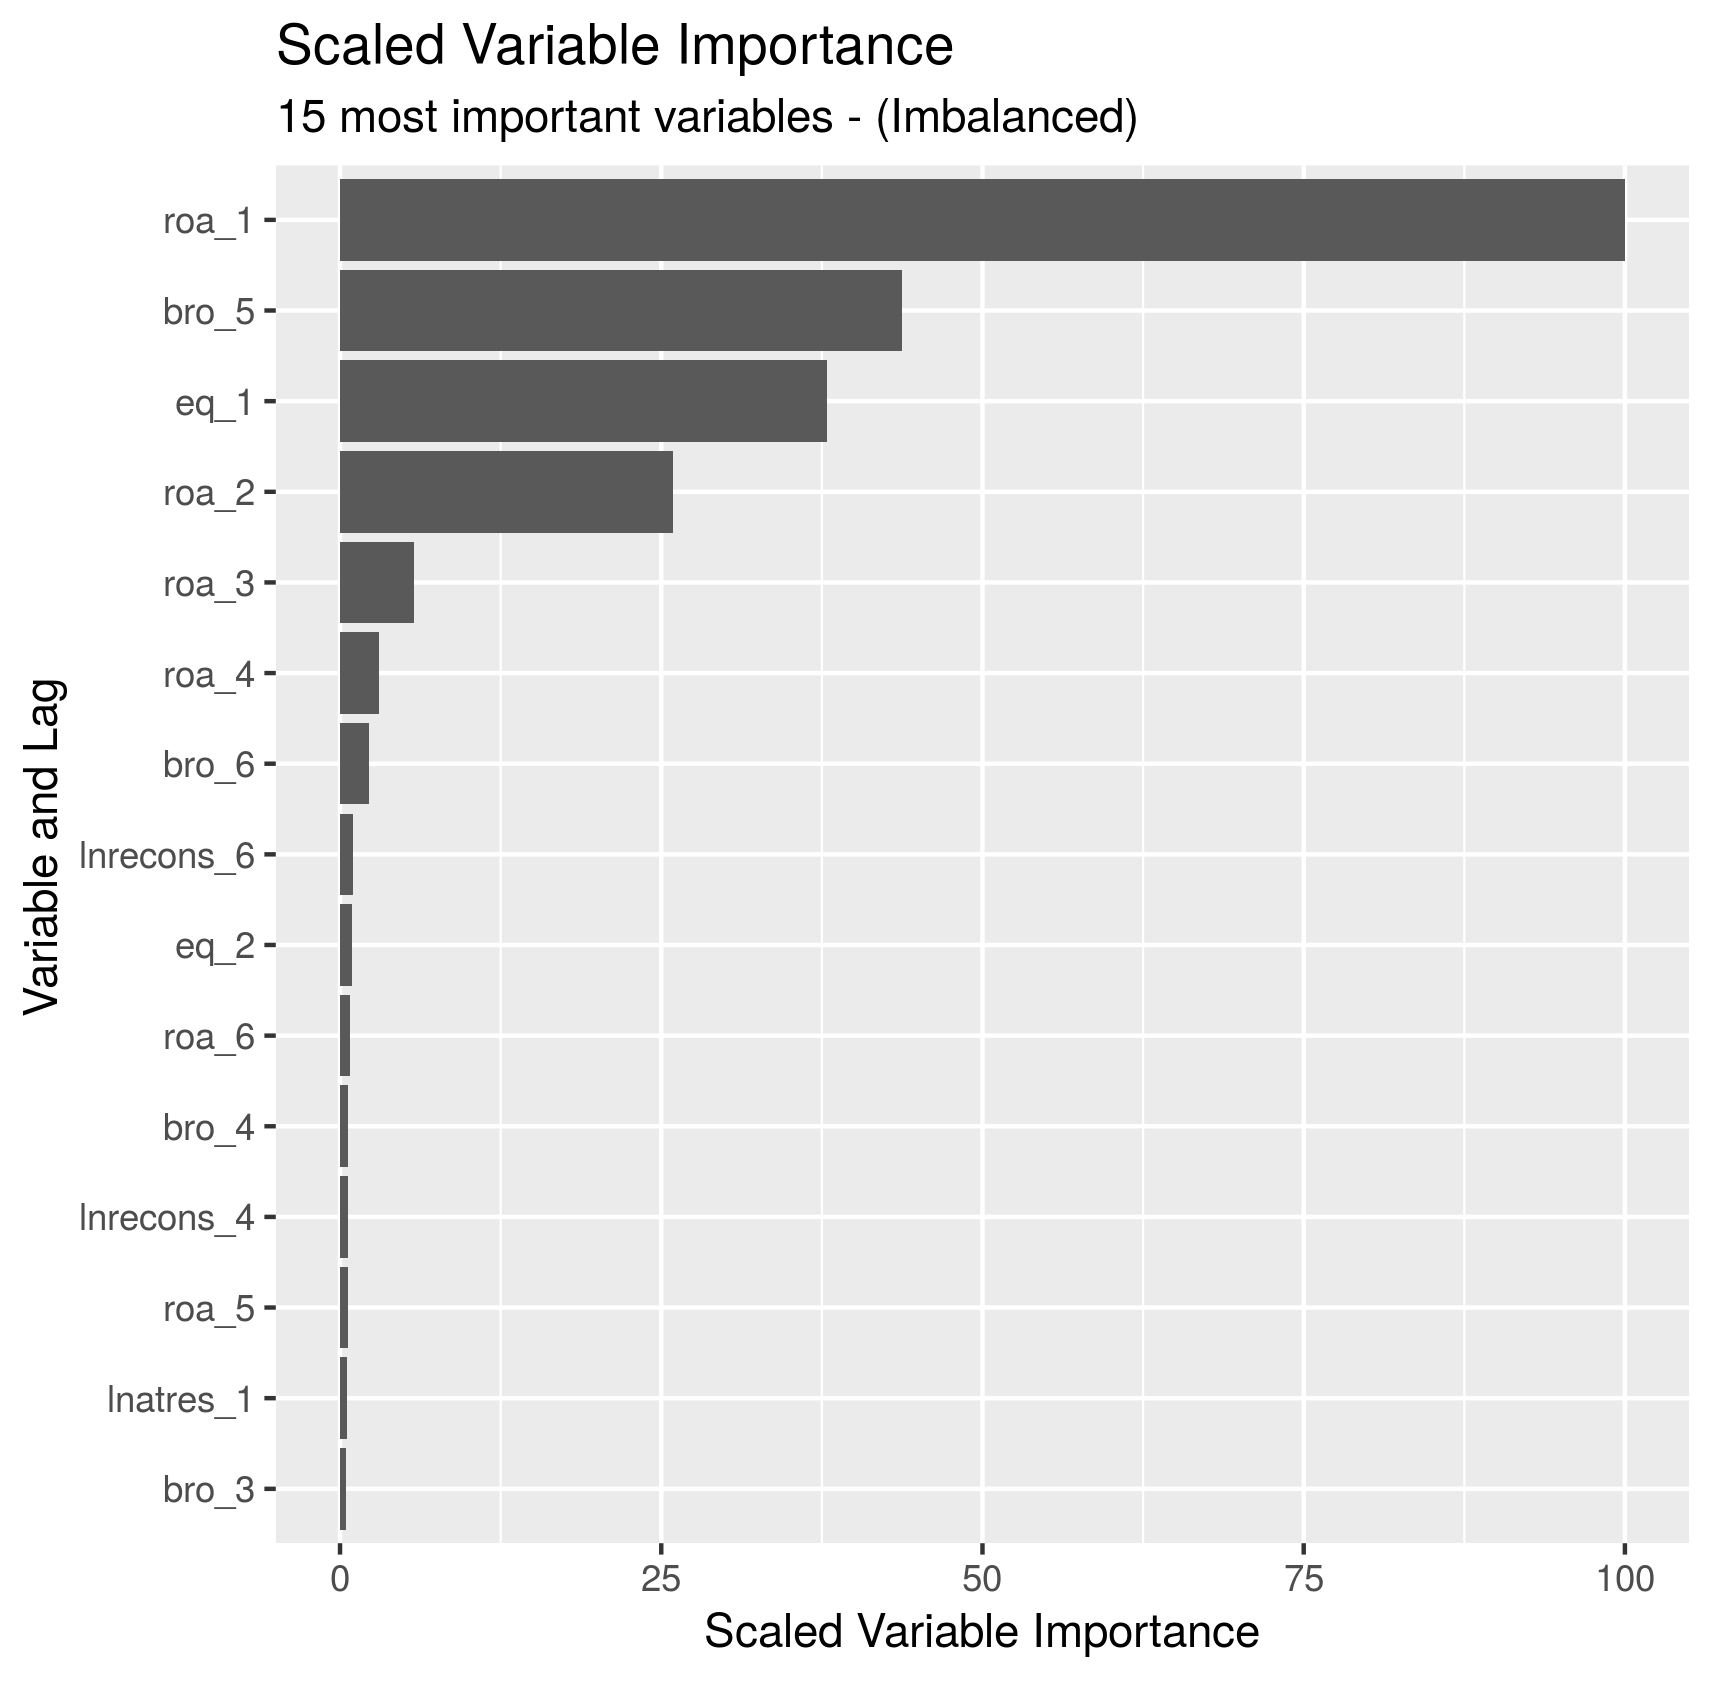
\includegraphics[width=\linewidth]{./graphics/var_imp/var_imp_imbalanced.png}
\caption{Imbalanced Model} \label{fig:a}
\end{subfigure}\hspace*{\fill}
\begin{subfigure}{0.48\textwidth}
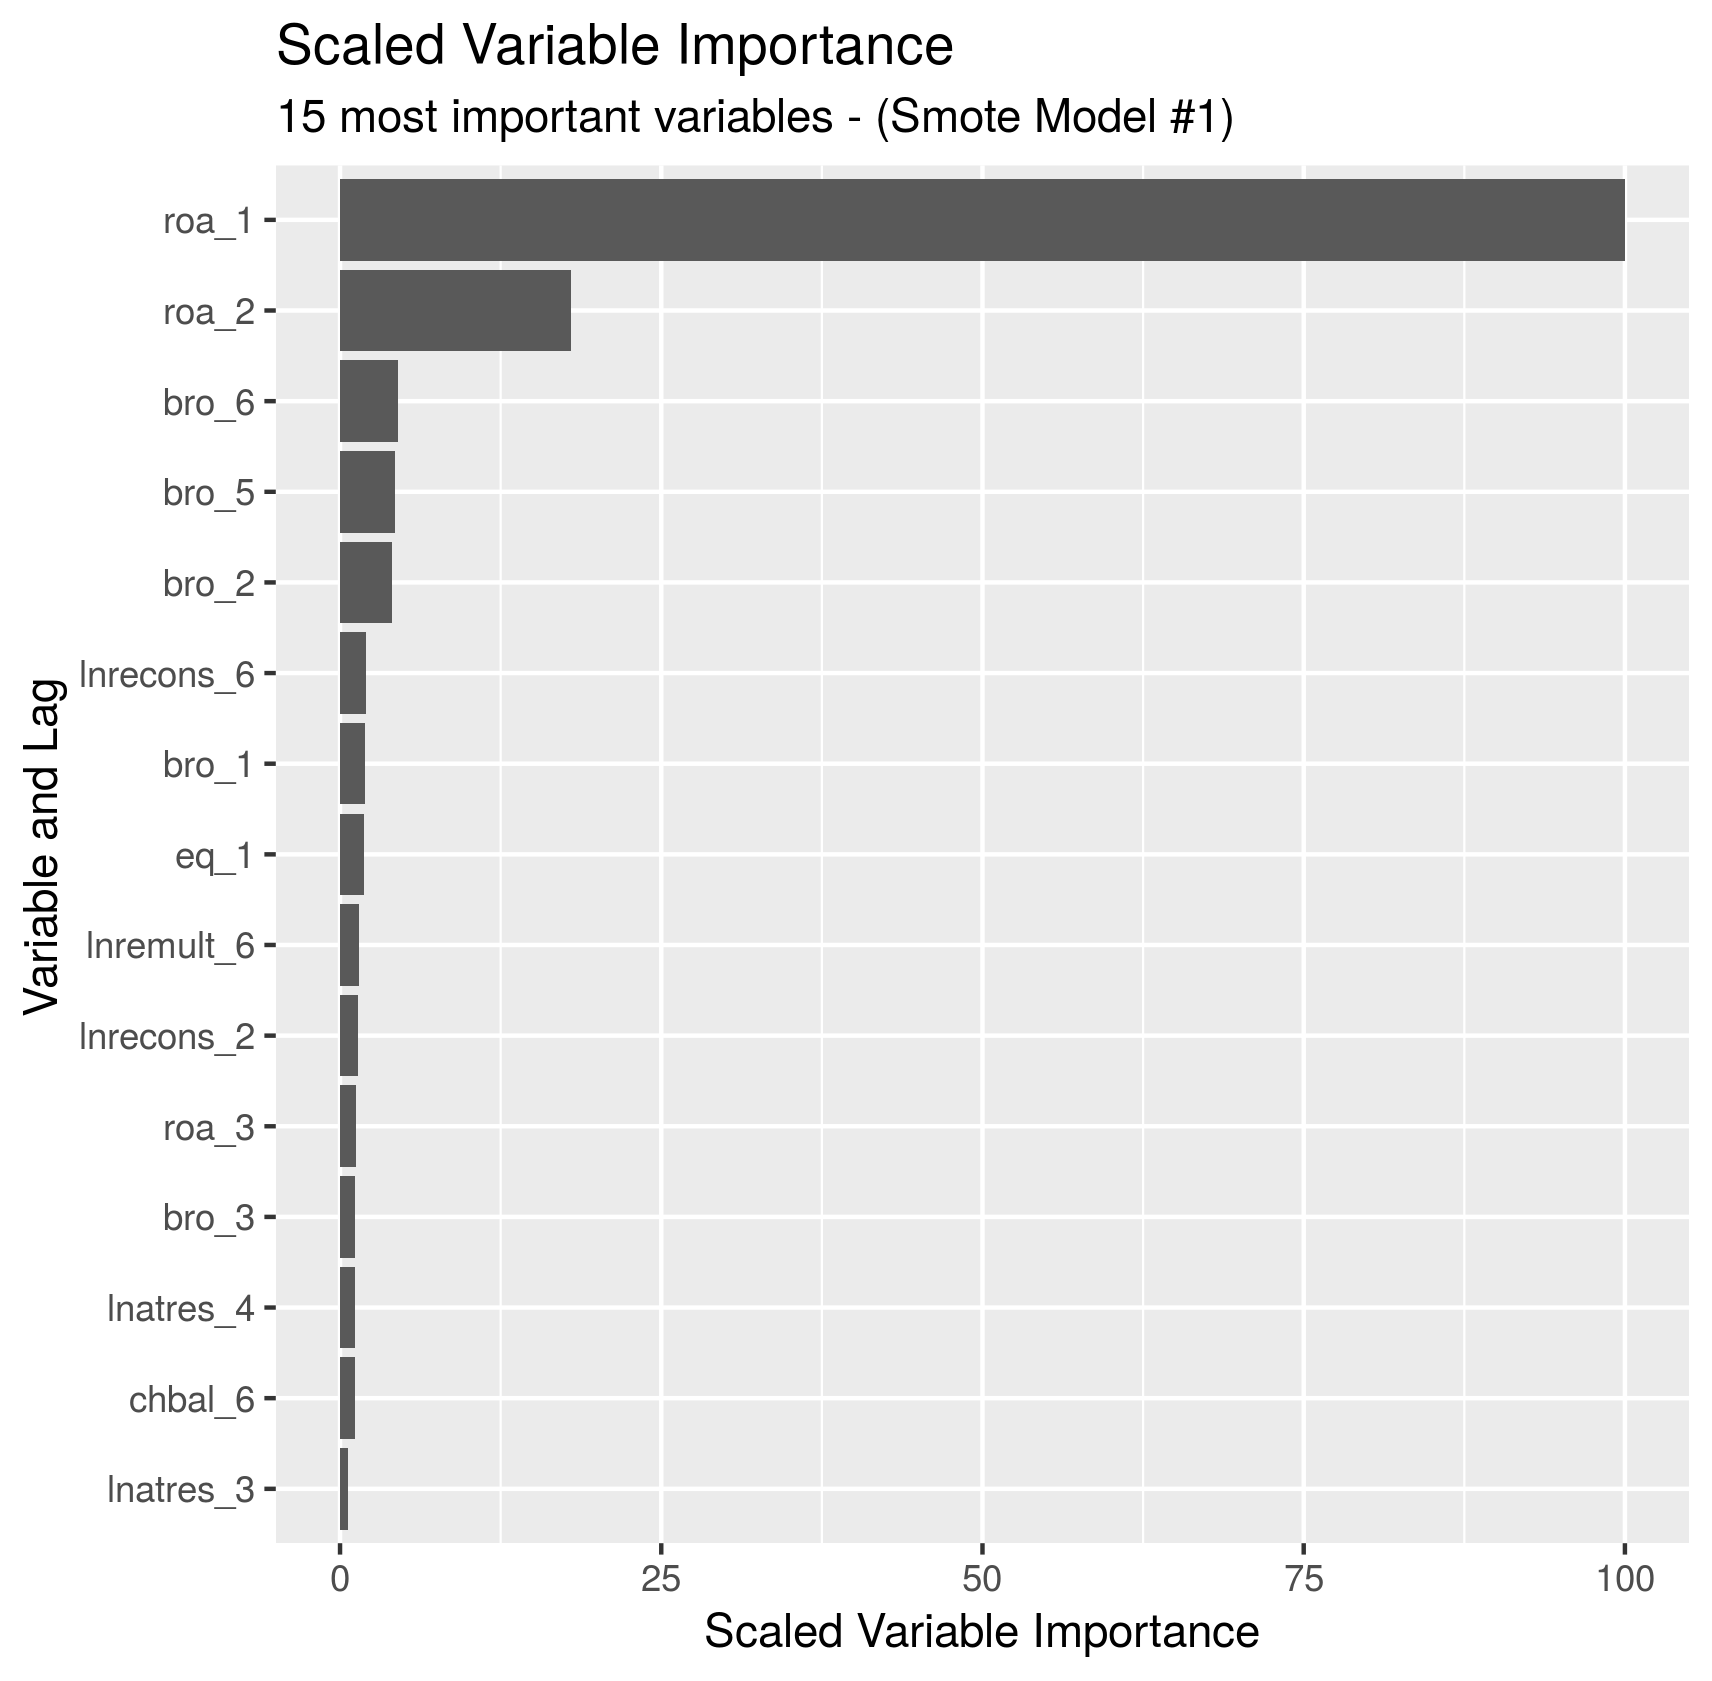
\includegraphics[width=\linewidth]{./graphics/var_imp/var_imp_smote1.png}
\caption{Smote Model \#1} \label{fig:a}
\end{subfigure}
\begin{subfigure}{0.48\textwidth}
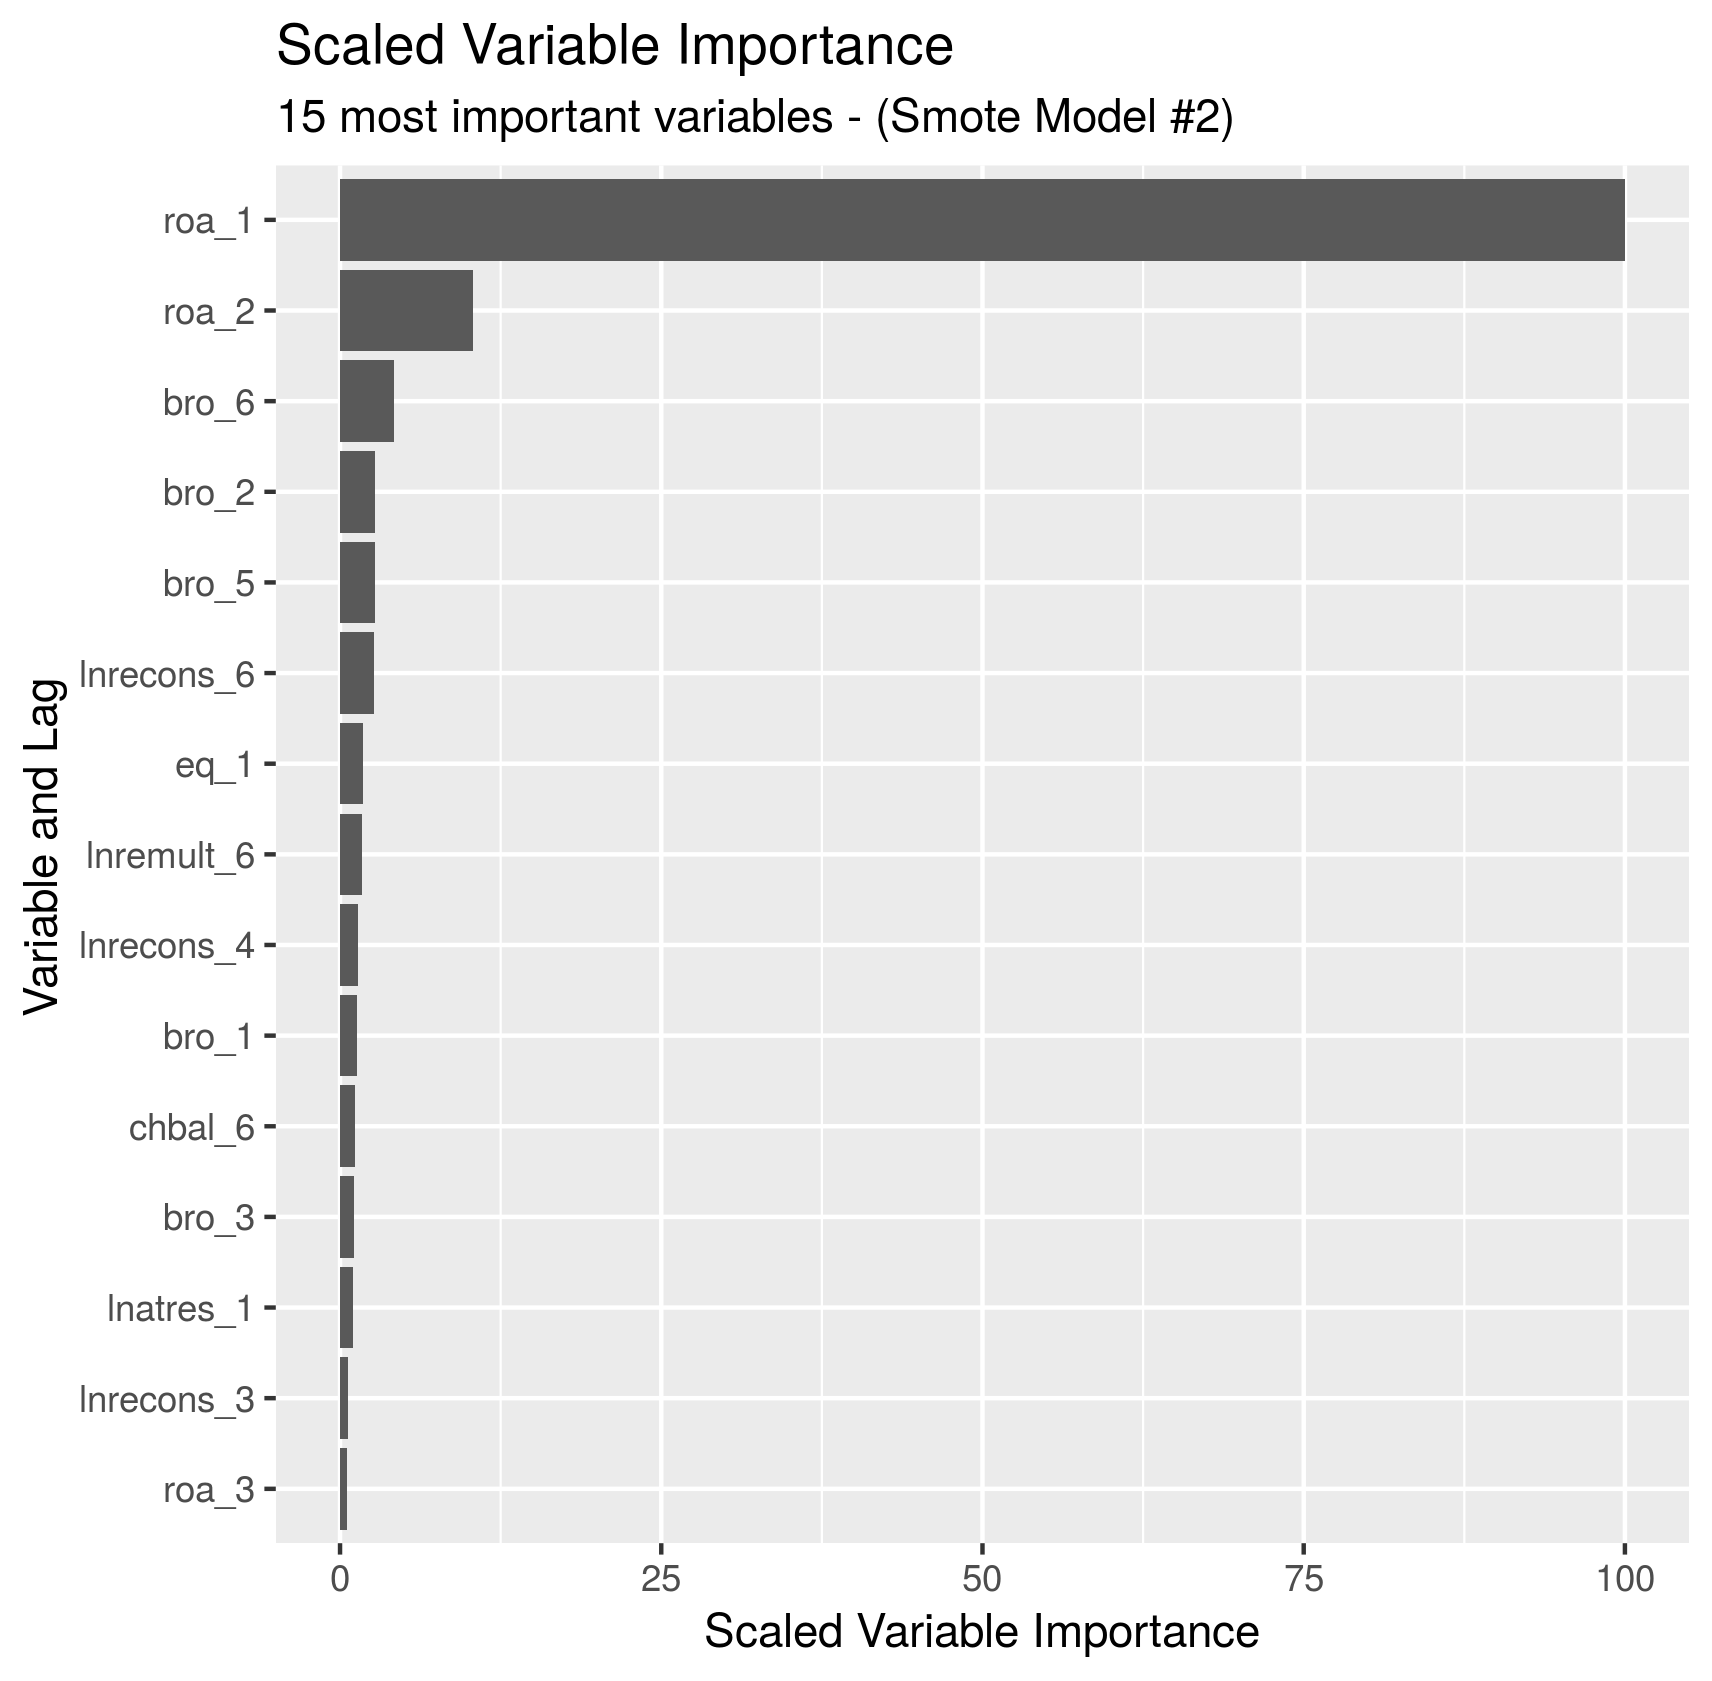
\includegraphics[width=\linewidth]{./graphics/var_imp/var_imp_smote2.png}
\caption{Smote Model \#2} \label{fig:a}
\end{subfigure}\hspace*{\fill}
\begin{subfigure}{0.48\textwidth}
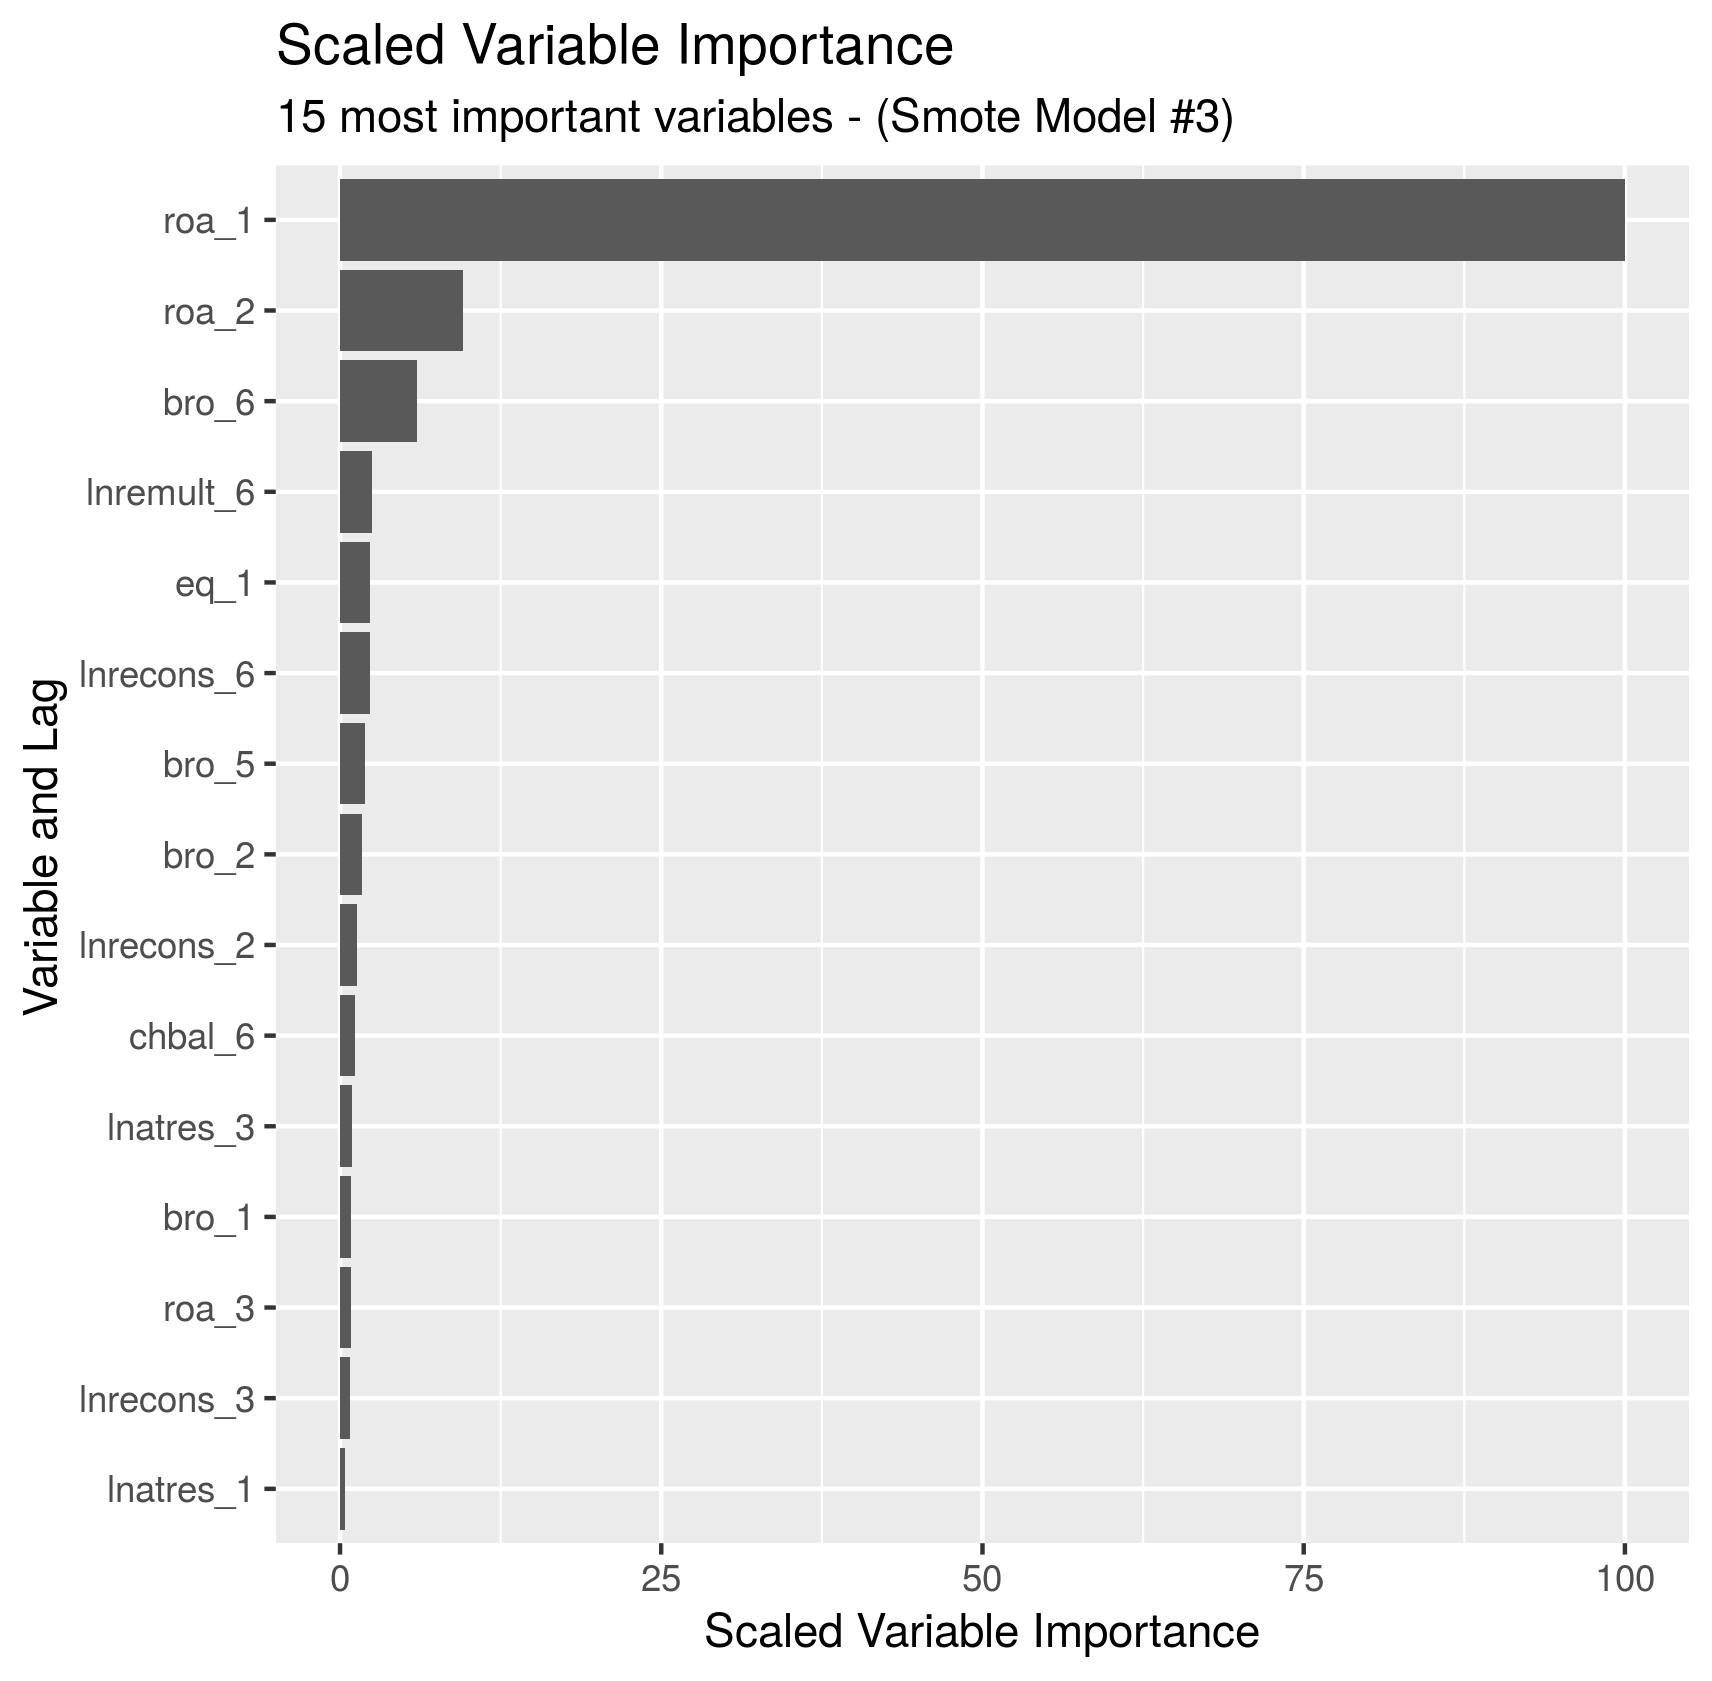
\includegraphics[width=\linewidth]{./graphics/var_imp/var_imp_smote3.png}
\caption{Smote Model \#3} \label{fig:a}
\end{subfigure}
\caption{Scaled Variable Importance for Top 15 Most Important Variables} \label{fig:2}
\end{figure}
\clearpage
\end{document}


 